\documentclass{book} % Definisi jenis dokumen

%%%%% Definisi paket-paket yang seharusnya digunakan %%%%%
\usepackage[utf8]{inputenc} % paket encoding input utf8
\usepackage[T1]{fontenc} % paket encoding huruf latin
\usepackage{tocbibind} % paket toc terdaftar dalam toc

%%%%% Definisi paket-paket yang digunakan sesuai kebutuhan %%%%%
\usepackage[yyyymmdd,hhmmss]{datetime} % paket tanggal-waktu
\usepackage{graphicx} % paket grafik/gambar
\usepackage[english]{babel} % paket modifikasi label/caption pada bahasa tertentu
\usepackage{geometry} % paket ukuran kertas dan margin
\usepackage{hyperref} % paket referensi url dan hyperlink
\usepackage{minted} % paket lingkungan kode sumber
\usepackage{xcolor} % paket definisi warna
\usepackage[os=win]{menukeys} % paket simbol keyboard standard Windows
\usepackage{amsmath} % paket formula matematis
\usepackage{enumitem} % paket enumeration lebih lanjut
\usepackage{subcaption} % paket untuk subfigure
\usepackage{booktabs} % paket garis tabel
\usepackage{multirow} % paket merge sel pada tabel
\usepackage{pgfplotstable} % paket impor csv menjadi tabel
\usepackage{tikz} % paket menggambar di latex
\usepackage{pgfplots} % paket plot csv via tikz
\usepackage[english]{babel} % paket bibliografi

%%%%% Pengaturan ukuran kertas dan margin %%%%%
\geometry{
	a4paper,
	left=10mm,
	right=10mm,
	top=15mm,
	bottom=15mm,
}

%%%%% Pengaturan perintah informasi perangkat lunak %%%%%
\newcommand{\ShowOsVersion}{
	\immediate\write18{\unexpanded{foo=`uname -sro` && echo "${foo}" > tmp.tex}}
	\input{tmp}\immediate\write18{rm tmp.tex}
}

\newcommand{\ShowTexVersion}{
	\immediate\write18{\unexpanded{foo=`pdflatex -version | head -n1 | cut -d' ' -f1,2` && echo "${foo}" > tmp.tex}}
	\input{tmp}\immediate\write18{rm tmp.tex}
}

%%%%% Mengganti label "Contents" ke "Daftar Isi" %%%%%
\addto\captionsenglish{\renewcommand{\contentsname}{Daftar Isi}}

%%%%% Mengganti label "Chapter" ke "Bab" %%%%%
\addto\captionsenglish{\renewcommand{\chaptername}{Bab}}

%%%%% Mengganti label "Figure" ke "Gambar" %%%%%
\addto\captionsenglish{\renewcommand{\figurename}{Gambar}}

%%%%% Mengganti label "List of Figures" ke "Daftar Gambar" %%%%%
\addto\captionsenglish{\renewcommand{\listfigurename}{Daftar Gambar}}

%%%%% Mengganti label "Table" ke "Tabel" %%%%%
\addto\captionsenglish{\renewcommand{\tablename}{Tabel}}

%%%%% Mengganti label "List of Tables" ke "Daftar Table" %%%%%
\addto\captionsenglish{\renewcommand{\listtablename}{Daftar Tabel}}

%%%%% Pengaturan teks link url/hyperlink %%%%%
\hypersetup{
	colorlinks=true, %set true if you want colored links
	linktoc=all,     %set to all if you want both sections and subsections linked
	linkcolor=blue,  %choose some color if you want links to stand out
	urlcolor=blue,   %url color
}

%%%%% Definisi warna baru %%%%%
\definecolor{LightGray}{gray}{0.95}

%%%%% Modifikasi kotak dan garis dari tikz %%%%%
\tikzstyle{squared} = [rectangle, rounded corners, minimum width=1cm, minimum height=0.5cm,text centered, draw=black]
\tikzstyle{connect1} = [ultra thick,->]
\tikzstyle{connect2} = [ultra thick,<->]

\begin{document}

    %%%%%%%%%%%%%%%%%%%%%%%%%%%%%%%%%%%%%%%%%%%%%%%%%%%%%%%%%%%%%%%%%

    \frontmatter % untuk halaman cover

    \begin{titlepage}
    	\addcontentsline{toc}{chapter}{Judul} % menambahkan judul ke Daftar Isi
    	
        \centering % untuk membuat tengah teks

        {
            \LARGE % pakai font besar
            \bf % pakai font BOLD
            Dasar Penulisan \LaTeX{} untuk Pemula
        }
		
		\bigskip
        {\Large \bf Achmadi ST MT}
        \vfill % menambahkan ruang kosong vertikal

		
\includegraphics[width=500pt]{images/leafcover}
		\vfill

		\raggedright
		\noindent Buku ini ditulis dengan:\\ % tanda \\ menambahkan garis baru
		OS : \ShowOsVersion \\
		TeX : \ShowTexVersion \\
		Update: {\today} at \currenttime\\
    \end{titlepage}

	%%%%%%%%%%%%%%%%%%%%%%%%%%%%%%%%%%%%%%%%%%%%%%%%%%%%%%%%%%%%%%%%%

	\newpage % halaman baru
	\tableofcontents % daftar isi
	\listoffigures % daftar gambar
	\listoftables % daftar table

	%%%%%%%%%%%%%%%%%%%%%%%%%%%%%%%%%%%%%%%%%%%%%%%%%%%%%%%%%%%%%%%%%

    \newpage
    \chapter{Disclaimer} % memulai chapter baru

    \LaTeX{} adalah proyek typesetting yang dimulai oleh \href{https://en.wikipedia.org/wiki/Leslie_Lamport}{Leslie Lamport}
    sekitar 40 tahun lalu dan sekarang dilanjutkan oleh \href{https://www.latex-project.org/}{latex-project.org}.

    \bigskip % baris kosong pemisah paragraf

    Buku tutorial ini disarikan dari \href{https://latex-tutorial.com/tutorials}{latex-tutorial.com}
    dan \href{https://www.overleaf.com/learn/latex/Tutorials}{overleaf.com} dengan alih bahasa dan penambahan konten sesuai selera penulis.

    %%%%%%%%%%%%%%%%%%%%%%%%%%%%%%%%%%%%%%%%%%%%%%%%%%%%%%%%%%%%%%%%%

	\newpage
	\chapter{Penggunaan Buku}

	\section{Umum} % memulai section baru
	Buku ini dibuat dengan tujuan penggunaan utama sebagai panduan digital untuk mempermudah search dan copy-paste.
	Anda tidak perlu mencetak buku ini ke bentuk kertas.
	Seluruh navigasi buku ini diharapkan menggunakan klik ke hyperlink di Daftar Isi,
	atau menggunakan tampilan \textbf{Index} yang tersedia di \textbf{SideBar} program pembaca PDF yang anda gunakan.

	\section{Petunjuk}
	Beberapa petunjuk yang digunakan di buku ini:
	\begin{itemize} % memulai lingkungan daftar tanpa angka (bullet list)
		\item \textbf{Cetak Tebal}: Menginformasikan identifier (keyword, opsi, nama file, dst) yang berada di suatu paragraf
		\item \textit{Cetak Miring}: Bersama simbol panah (->) dan simbol lain, menginformasikan langkah-langkah klik menu/tombol.
		\item \textbf{TIPS:} Menginformasikan hal-hal yang dapat membantu atau pengetahuan tambahan.
		\item \textbf{PERINGATAN:} Menginformasikan hal-hal yang bener-benar harus diperhatikan.
	\end{itemize}

	\section{Penulisan Kode}
	Untuk penulisan kode, akan digunakan sebagai berikut:

    % lingkungan penulisan kode sumber
    \begin{minted}[frame=lines,framesep=2mm,fontsize=\normalsize,bgcolor=LightGray]{tex}
\begin{enumerate}
    \item Pertama
    \item Kedua
\end{enumerate }
    \end{minted}

    \section{Kode Sumber Dokumen}

    Seluruh isi buku ini juga ditulis dengan \LaTeX{}, sehingga jika dibutuhkan contoh, dapat melihat
    kode sumber dokumen ini yang tersedia di \href{https://github.com/mekatronik-achmadi/my_latexbook/blob/master/Modul/LaTex/latex_beginner.tex}{GitHub Penulis}.

    \bigskip

    Selain itu, website seperti \href{https://www.overleaf.com/}{Overleaf.com} menyediakan beragam tutorial dan contoh siap pakai.

    %%%%%%%%%%%%%%%%%%%%%%%%%%%%%%%%%%%%%%%%%%%%%%%%%%%%%%%%%%%%%%%%%

    \mainmatter % pindah format halaman dari romawi ke angka (konten utama)

    \newpage
    \chapter{Introduksi}

    \section{Apa itu \LaTeX{}}

    \LaTeX{} adalah bahasa markup (seperti HTML dan Markdown) untuk typeset (mengatur penulisan) dokumen.
    Format berkas dokumen \LaTeX{} umumnya berupa berkas teks yang disimpan di suatu folder
    bersamaan dengan berkas pendukung lain (seperti gambar, pdf, dan sebagainya).
    Berkas teks ini kemudian dikompilasi menjadi berkas akhir (umumnya PDF atau DVI).

    \LaTeX{} sangat populer digunakan untuk antara lain:
    \begin{itemize}
        \item Jurnal, paper, atau artikel akademik.
        \item Laporan Teknis.
        \item Buku atau Novel.
        \item Presentasi.
    \end{itemize}

    \section{Contoh kode \LaTeX{}}

    Secara umum, \LaTeX{} ditulis dalam bentuk kode tag/markup dan karakter teks seperti pada umumnya.
    Berikut contoh kode \LaTeX{} dan hasilnya:

    \begin{minted}[frame=lines,framesep=2mm,fontsize=\normalsize,bgcolor=LightGray]{tex}
\begin{center}
    Hello World, \LaTeX{}
\end{center}
    \end{minted}

    Hasil kode di atas akan menghasilkan sebagai berikut:
    \begin{center}
        Hello World, \LaTeX{}
    \end{center}

    \section{Komentar dalam LaTeX}

    Selayaknya bahasa pemrograman pada umumnya, LaTeX mengenal mekanisme komentar yang tidak akan dikompilasi ke dokumen akhir.
    Komentar dalam latex adalah komentar per baris yang dimulai dengan karakter persen '\%'.

    Sebagai contoh:

    \begin{minted}[frame=lines,framesep=2mm,fontsize=\normalsize,bgcolor=LightGray]{tex}
\begin{itemize}
    \item First % Ini pertama
    \item Second % Ini kedua
\end{itemize}
    \end{minted}

    Yang akan menghasikan (tanpa ada konten setelah tanda persen) :

    \begin{itemize}
        \item First % Ini pertama
        \item Second % Ini kedua
    \end{itemize}

	\newpage
    Jika dibutuhkan menulis simbol persen, ditambahkan simbol backslash ('\textbackslash').
    Contohnya:

    \begin{minted}[frame=lines,framesep=2mm,fontsize=\normalsize,bgcolor=LightGray]{tex}
Uang senilai 50\% dari Rp.1000 adalah Rp.500
    \end{minted}

    Menghasilkan: \\
    Uang senilai 50\% dari Rp.1000 adalah Rp.500
    
    \bigskip
    
    \textbf{TIPS:} karakter khusus seperti '\%', '\{', '\}', '\&', dst dapat digunakan sebagai teks biasa dengan ditambahkan
    '\textbackslash', sehingga ditulis sebagai '\textbackslash\%', '\textbackslash\{', '\textbackslash\}', '\textbackslash\&', dst. 

    \section{Apakah \LaTeX{} termasuk Word-Processor}

    \LaTeX{} sama sekali \textbf{BUKAN} word-processor seperti MS-Word, LO-Writer, OO-Document, Google-Doc, atau yang serupa.

    \bigskip

    Perbedaan mendasar adalah:
    \begin{itemize}
        \item Word-Processor menganut paradigma WYSIWYG,
        sedangkan \LaTeX{} adalah markup dan typesetting yang perlu dikompilasi terlebih dahulu.

        \item Word-Processor modern membutuhkan perangkat layout seperti mouse/touchpad,
        sedangkan \LaTeX{} murni programmatikal teks.
    \end{itemize}

    \bigskip

    Keuntungan Word-processor dibandingkan \LaTeX{}:
    \begin{itemize}
        \item Dokumen workflow yang telah dikenalkan sejak kita SD.
        \item Penguna lebih banyak dan lebih umum.
    \end{itemize}

    \bigskip

    Keuntungan \LaTeX{} dibandingkan Word-Processor:
    \begin{itemize}
    	\item Format dan paket \LaTeX{} bersifat gratis dan open-sources.
        \item Satu template dapat digunakan berkali-kali.
        \item Tampilan dokumen diatur template, sehingga penulis bisa fokus pada konten saja.
        \item Hasil penulisan format rumus kompleks bagus.
        \item Hasil penulisan kode programming bagus.
        \item Hasil penulisan bibliografi akademik bagus.
        \item Format berkas adalah teks, sehingga mudah untuk editting (tidak butuh CPU/GPU/RAM besar)
        dan dapat direkam content-tracking atau source-code manager seperti Git, CVS, atau Mercurial.
    \end{itemize}

	%%%%%%%%%%%%%%%%%%%%%%%%%%%%%%%%%%%%%%%%%%%%%%%%%%%%%%%%%%%%%%%%%

	\chapter{Installasi}

	Mengingat \LaTeX{} yang bersifat open-sources, maka dapat dipastikan \LaTeX{} tersedia di major-OS seperti GNU/Linux, Windows, dan MacOS.
	Selain paket offline, tersedia pula \LaTeX{} editor dan builder online.

	\section{Paket Offline}

	Keuntungan instalasi paket offline antara lain:

	\begin{itemize}
		\item Tidak selalu membutuhkan koneksi internet.
		\item Kompilasi PDF cenderung lebih cepat.
		\item Modifikasi dan pengaturan dapat permanen.
	\end{itemize}

	\subsection{GNU/Linux}

	\subsubsection{TexLive}

	Distribusi \LaTeX{} yang saat ini (tahun 2022) umum digunakan adalah \href{https://www.tug.org/texlive/}{TeX Live}.
	Distribusi ini telah tersedia di banyak distro GNU/Linux dan dapat diinstall dari repository masing-masing melalui perintah di terminal.
	Konsultasikan dengan admin GNU/Linux anda jika kesulitan menginstal.

	Contoh instalasi disini akan digunakan contoh pada ArchLinux/Manjaro, namun umumnya serupa untuk distro OS GNU/Linux lain seperti Ubuntu atau Fedora.

	Perintah di terminal untuk instalasi:
	\begin{minted}[frame=lines,framesep=2mm,fontsize=\normalsize,bgcolor=LightGray]{bash}
$> sudo pacman -S texlive-formatsextra texlive-bibtexextra \
texlive-latexextra texlive-publishers texlive-fontsextra \
texlive-pictures texlive-pstricks texlive-science texlive-core \
texlive-bin latex2html latex2rtf dblatex minted biber pdftk
	\end{minted}

	Untuk paket penuh lengkap akan mendownload setidaknya 800MB dan instalasi sekitar 2.5GB.

	\bigskip

	Kemudian untuk pilihan editor, berikut tersedia beberapa pilihan

	\subsubsection{TexStudio}

	TexStudio adalah lingkungan terintegrasi untuk mengerjakan dokumen \LaTeX{}.
	TexStudo bersifat gratis dan open-sources.
	Fitur utama TexStudio antara lain:
	\begin{itemize}
		\item Syntax-Highlighting.
		\item Cek Reference/Bibliography.
		\item Auto-Completion yang sangat lengkap.
	\end{itemize}

	Perintah instal di terminal:

	\begin{minted}[frame=lines,framesep=2mm,fontsize=\normalsize,bgcolor=LightGray]{bash}
$> sudo pacman -S texstudio
	\end{minted}

	Instalasi akan berkisar 500MB (ditambah instalasi pustaka Qt5 sebagai toolkit GUI).

	\newpage
	\begin{figure}[!ht]
% lingkungan untuk gambar
		\centering
		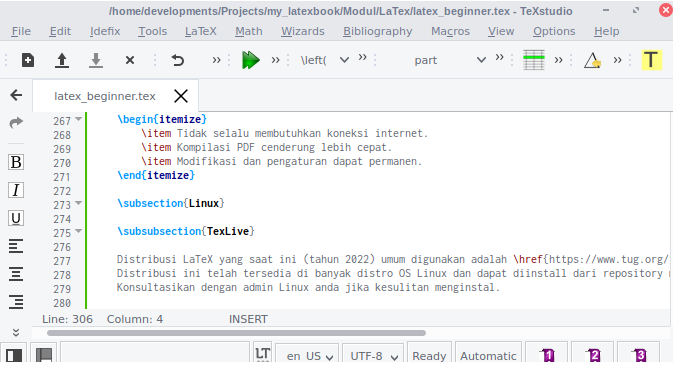
\includegraphics[width=400pt]{images/texstudio}
		\caption{Contoh TexStudio}
	\end{figure}

	\textbf{TIPS:} Untuk perintah kompilasi, pastikan terdapat opsi \textbf{-shell-escape}.
	Jika belum, dapat ditambahkan opsi tersebut pada menu \textit{Options} -> \textit{Configure TexStudio}.
	Kemudian pilih tab \textit{Commands}.

	\begin{figure}[!ht]
% lingkungan untuk gambar
		\centering
		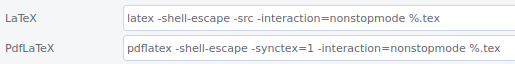
\includegraphics[width=450pt]{images/texstudio_shellescape}
		\caption{Opsi Shell Escape}
	\end{figure}

	\subsubsection{Visual Studio Code}

	Visual Studio Code adalah editor pemrograman multiguna buatan Microsoft yang fungsi dan fiturnya dapat ditambahkan dengan segudang ekstensi.
	Untuk mengerjakan \LaTeX{}, dapat digunakan ekstensi \href{https://github.com/James-Yu/LaTeX-Workshop}{LaTeX-Workshop}.

	Untuk instalasi di ArchLinux/Manjaro, dapat digunakan paket VSCodium di AUR:\\
	\url{https://aur.archlinux.org/packages/vscodium-bin/}.

	\begin{figure}[!ht]
		\centering
		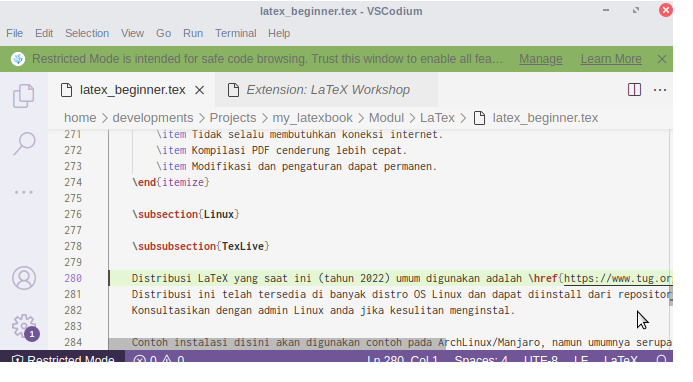
\includegraphics[width=400pt]{images/vscodium}
		\caption{Contoh VSCodium}
	\end{figure}

	Kemudian ekstensi LaTeX-Workshop dapat diinstal di program VSCodium sendiri pada menu \textit{View} -> \textit{Extension}.

	\newpage

	\subsubsection{Makefile}

	Khusus GNU/Linux, pada dasarnya dapat digunakan editor teks apapun (termasuk editor CLI seperti Vim, Nano, atau Emacs).
	Untuk mengkompilasi berkas \LaTeX{} (umumnya berekstensi \textbf{*.tex}), dapat digunakan perintah di terminal seperti:

	\begin{minted}[frame=lines,framesep=2mm,fontsize=\normalsize,bgcolor=LightGray]{bash}
$> pdflatex -shell-escape -synctex=1 -interaction=nonstopmode dokumen.tex
	\end{minted}

	\textbf{TIPS:} Jika dokumen menggunakan Table of Content atau Index, maka perintah di atas dapat dijalankan dua kali untuk update TOC.

	Untuk mempermudah eksekusi berkali-kali, dapat digunakan program GNU Make.
	Jika belum tersedia, dapat diinstal dengan perintah:

	\begin{minted}[frame=lines,framesep=2mm,fontsize=\normalsize,bgcolor=LightGray]{bash}
$> sudo pacman -S make
	\end{minted}

	Kemudian buat berkas bernama \textbf{Makefile} berikut dan simpan di folder yang sama dengan berkas *.tex dan berkas-berkas pendukungnya.

	\begin{minted}[frame=lines,framesep=2mm,fontsize=\normalsize,bgcolor=LightGray]{make}
TEXCC=pdflatex
TEXFLAGS=-shell-escape -synctex=1 -interaction=nonstopmode

all:
	for texfiles in `ls -1 *.tex`;do $(TEXCC) $(TEXFLAGS) $$texfiles;done
	for texfiles in `ls -1 *.tex`;do $(TEXCC) $(TEXFLAGS) $$texfiles;done # run twice for TOC

clean:
	rm -f *.log *.toc *.synctex.gz *.aux
	rm -f *.out *.bbl *.blg *.lof
	rm -f *.pdf
	rm -rf ./_minted*
	\end{minted}

	Selanjutnya untuk kompilasi dokumen, tinggal digunakan perintah terminal (pada alamat dimana berkas *.tex berada):

	\begin{minted}[frame=lines,framesep=2mm,fontsize=\normalsize,bgcolor=LightGray]{bash}
$> make all
	\end{minted}

	Dan untuk membersihkan, digunakan perintah:

	\begin{minted}[frame=lines,framesep=2mm,fontsize=\normalsize,bgcolor=LightGray]{bash}
$> make clean
	\end{minted}

	\subsection{Windows}
	
	Menyusul setelah internet kampus nyala

	\subsubsection{TexLive}
	
	Menyusul setelah internet kampus nyala
	
	\subsubsection{TexStudio}
	
	Menyusul setelah internet kampus nyala
	
	\subsubsection{Visual Studio Code}
	
	Menyusul setelah internet kampus nyala

	\subsection{MacOS}

	Penulis tidak punya akses terhadap sistem operasi MacOS maupun turunan Darwin/BSD lainnya,
	sehingga tidak dapat mencoba sendiri proses instalasinya.

	Namun tersedia banyak tutorial untuk instalasi paket TexLive dan TexStudio/VSCodium untuk MacOS/Darwin di internet.
	Silahkan cari sendiri.

	\section{Editor Online}

	Keuntungan editor \LaTeX{} online antara lain:
	\begin{itemize}
		\item Tidak perlu instal apa pun.
		\item Dapat digunakan di komputer mana pun.
		\item Hanya membutuhkan koneksi internet dan webbrowser yang mendukung Javascript (semisal Firefox).
	\end{itemize}

	Salah satu yang direkomendasikan adalah \href{https://www.overleaf.com/project}{Overleaf Online Editor}.
	Cukup registrasi gratis dengan email Google, maka sudah dapat digunakan dengan akun gratis.

	\begin{figure}[!ht]
		\centering
		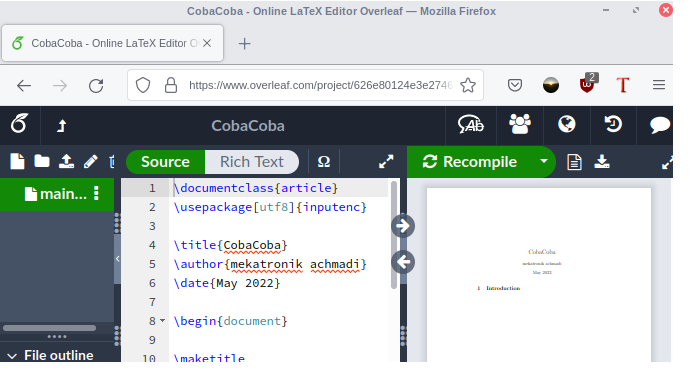
\includegraphics[width=400pt]{images/overleaf}
		\caption{Contoh online editor Overleaf}
	\end{figure}

	\section{Acuan Panduan}

	Untuk kebutuhan panduan disini, digunakan TeXLive offline dengan editor TexStudio di GNU/Linux (ArchLinux) sebagai acuan.
	Anda dapat mengikuti tutorial ini jika anda menggunakan Windows tanpa perlu ada penyesuaian apa pun.

	\bigskip

	Untuk editor online, anda tetap dapat mengikuti dengan sedikit banyak penyesuaian yang mungkin saja tidak dijelaskan di panduan ini.
	
    %%%%%%%%%%%%%%%%%%%%%%%%%%%%%%%%%%%%%%%%%%%%%%%%%%%%%%%%%%%%%%%%%

	\chapter{Dasar Dokumen \LaTeX{}}

	Bab ini menjelaskan dasar penulisan dokumen \LaTeX{} yang berlaku secara umum untuk semua jenis dokumen \LaTeX{}.

	\section{Kerangka Dasar}

	Berikut dijelaskan kerangka dasar yang membangun suatu dokumen \LaTeX{}.

	\subsection{Pola Struktur}

	Struktur dasar dokumen umumnya seperti berikut:

	\begin{minted}[frame=lines,framesep=2mm,fontsize=\normalsize,bgcolor=LightGray]{tex}
\documentclass{class} % Definisi jenis dokumen

\usepackage{package} % Memanggil paket definisi tambahan

% Pengaturan tambahan di area ini

\begin{document} % awal dokumen

	% konten dokumen di area ini

\end{document} % akhir dokumen
	\end{minted}

	Beberapa pilihan \textbf{class} yang dapat dipakai antara lain:
	\begin{itemize}
		\item \textbf{article}. Untuk dokumen pendek dan artikel/paper. Paling umum digunakan.
		\item \textbf{report}. Untuk dokumen panjang dan jurnal/disertasi.
		\item \textbf{book}. Untuk membuat buku yang memiliki bab (chapter).
		\item \textbf{letter}. Untuk dokumen surat pemberkasan.
		\item \textbf{beamer}. Untuk membuat slide presentasi.
	\end{itemize}

	\subsection{Contoh Minimum}

	Berikut contoh minimum dokumen \LaTeX{} yang dapat dikompilasi ke format PDF.
	Simpan dengan nama \textbf{helloworld.tex}

	\begin{minted}[frame=lines,framesep=2mm,fontsize=\normalsize,bgcolor=LightGray]{tex}
\documentclass{article}

\usepackage[utf8]{inputenc} %  % paket encoding input utf8
\usepackage[T1]{fontenc} %  % paket encoding huruf latin
\usepackage{tocbibind} % paket toc terdaftar dalam toc

\begin{document}
	Hello World, \LaTeX{}
\end{document}
	\end{minted}

	\newpage
	\section{Kompilasi PDF}

	Berikut beberapa metode kompilasi ke PDF berdasarkan editor yang digunakan.

	\bigskip

	\textbf{PERINGATAN:} Pada langkah ini diasumsikan bahwa paket offline TexLive dan program kompiler \textbf{pdflatex} telah siap digunakan.
	Bagian ini tidak mencantumkan langkah-langkah editor online.

	\subsection{TexStudio}

	Kompilasi PDF dapat dilakukan dengan:
	\begin{itemize}
		\item Klik menu \textit{Tools} -> \textit{Build and View}.
		\item Atau tekan tombol \keys{F5}.
		\item Tunggu beberapa saat hingga muncul tampilan preview PDF pada TexStudio.
		\item Dokumen \textbf{helloworld.pdf} akan muncul di folder yang sama.
	\end{itemize}

	\begin{figure}[!ht]
		\centering
		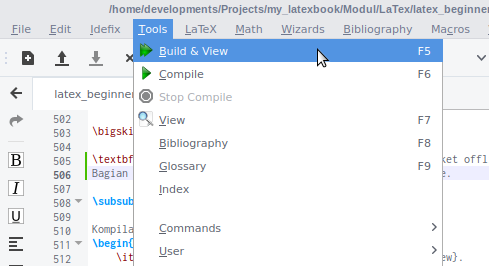
\includegraphics[width=250pt]{images/texstudio_compile}
		\caption{Build dengan TexStudio}
	\end{figure}

	\subsection{Visual Studio Code}

	Kompilasi PDF dilakukan di terminal VSCode.
	Langkahnya adalah:

	\begin{itemize}
		\item Klik menu \textit{Terminal} -> \textit{New Terminal} (jika belum ada terminal tab terbuka).
		\item Pastikan alamat terminal sama dengan folder tempat berkas tex berada.
		Anda dapat cek keberadaan berkas terminal dengan perintah:
		\begin{minted}[frame=lines,framesep=2mm,fontsize=\normalsize,bgcolor=LightGray]{bash}
$> ls | grep helloworld.tex
		\end{minted}
		\item Masukkan perintah berikut:
	\begin{minted}[frame=lines,framesep=2mm,fontsize=\normalsize,bgcolor=LightGray]{bash}
$> pdflatex -shell-escape -synctex=1 -interaction=nonstopmode helloworld.tex
	\end{minted}
		\item Tunggu beberapa saat hingga muncul pesan "Output written on helloworld.pdf".
		\item Dokumen \textbf{helloworld.pdf} akan muncul di folder yang sama.
	\end{itemize}

	\textbf{TIPS:} Karena kompilasi dilakukan di terminal, jika menggunakan GNU/Linux maka dapat pula menggunakan
	metode Makefile seperti yang dijelaskan sebelumnya.

	\newpage
	\begin{figure}[!ht]
		\centering
		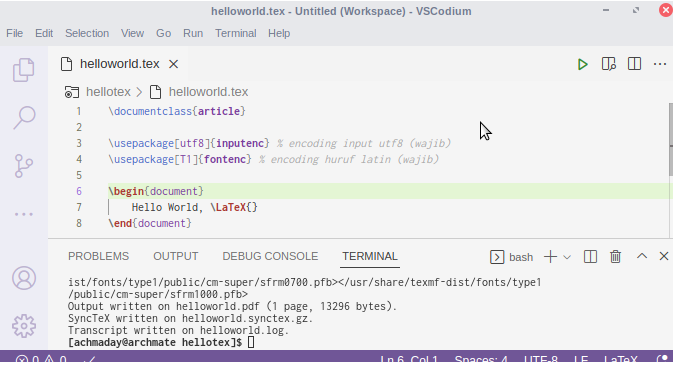
\includegraphics[width=300pt]{images/vscode_compile}
		\caption{Build dengan VSCode}
	\end{figure}

	\section{Tag/Environment}
	
	Kontrol dan layout dokumen dituangkan dalam tanda Tag dan Enviroment
	
	\subsection{Tag}
	
	Tag adalah kontrol dimulai dengan karakter backslash ('\textbackslash') kemudian diikuti perintah yang dikenali kompiler dokumen.
	Tag merupakan bentuk dasar semua penulisan dokumen \LaTeX.
	
	\bigskip
	
	Sebagai contoh, untuk logo \LaTeX{} seperti ini, digunakan tag \textbf{LaTeX} yang diawali backslash ('\textbf{\textbackslash}') agar dikenali sebagai tag oleh kompiler.
	
	\begin{minted}[frame=lines,framesep=2mm,fontsize=\normalsize,bgcolor=LightGray]{tex}
\LaTeX % contoh tag yang di awali '\'
	\end{minted}
	
	maka akan menghasilkan: \LaTeX.
	
	Selain itu, tag dengan tanda kurung kurawal ('\{\}') dapat digunakan untuk modifikasi teks.
	Sebagai contoh modikasi style font:
	
	\begin{minted}[frame=lines,framesep=2mm,fontsize=\normalsize,bgcolor=LightGray]{tex}
Ini normal \\
\textbf{Ini Bold} \\
\textit{Ini Italic}
	\end{minted}

	akan menghasilkan:\\
	Ini normal \\
	\textbf{Ini Bold} \\
	\textit{Ini Italic}
	
	\bigskip
	
	\textbf{TIPS:} Simbol dobel blackslash ('\textbackslash\textbackslash') adalah tag untuk menambahkan baris baru.

	\subsection{Environment}
	
	Environment atau lingkungan adalah metode mengurung teks dalam suatu pengaturan khusus
	yang hanya berlaku di dalam lingkungan itu sendiri.
	
	\bigskip
	
	Semua lingkungan dimulai oleh tag \textbf{begin} dan diakiri \textbf{end}.
	Untuk lingkungan \textbf{document} harus digunakan sebagai lingkungan tertinggi (paling luar).
	
	\newpage
	Pola umum penggunaan lingkungan adalah seperti ini:
	
	\begin{minted}[frame=lines,framesep=2mm,fontsize=\normalsize,bgcolor=LightGray]{tex}
\begin{document}
	
	\begin{lingkungan1}
		konten1
	\end{lingkungan1}

	\begin{lingkungan2}
		konten2
	\end{lingkungan2}

	\begin{lingkungan3}
		konten3
	\end{lingkungan3}

\end{document}
	\end{minted}

	Sebagai contoh, untuk pengaturan menengahkan teks:
	
	\begin{minted}[frame=lines,framesep=2mm,fontsize=\normalsize,bgcolor=LightGray]{tex}
Baris pertama untuk normal.\\
Baris kedua untuk normal. \\
Baris ketiga untuk normal.

\begin{center}
	Baris pertama untuk tengah.\\
	Baris kedua untuk tengah. \\
	Baris ketiga untuk tengah.
\end{center}

Baris pertama untuk kembali normal.\\
Baris kedua untuk kembali normal. \\
Baris ketiga untuk kembali normal.

\begin{flushright}
	Baris pertama untuk kanan.\\
	Baris kedua untuk kanan. \\
	Baris ketiga untuk kanan.
\end{flushright}
	\end{minted}

	akan menghasilkan:
	
	\bigskip
	
	Baris pertama untuk normal.\\
	Baris kedua untuk normal. \\
	Baris ketiga untuk normal.
	
	\begin{center}
		Baris pertama untuk tengah.\\
		Baris kedua untuk tengah. \\
		Baris ketiga untuk tengah.
	\end{center}
	
	Baris pertama untuk kembali normal.\\
	Baris kedua untuk kembali normal. \\
	Baris ketiga untuk kembali normal.

	\begin{flushright}
		Baris pertama untuk kanan.\\
		Baris kedua untuk kanan. \\
		Baris ketiga untuk kanan.
	\end{flushright}

	\newpage
	\section{Strukturisasi}
	
	Strukturisasi mengacu kepada penggunaan tag \textbf{chapter}, \textbf{section}, \textbf{subsection}, dan seterusnya.
	Fungsinya adalah untuk membagi dokumen sehingga pembahasan lebih terstruktur.
	Terdapat pula tag \textbf{paragraph} dan \textbf{subparagraph},
	namun kedua tag ini tidak terdaftar pada TOC sehingga tidak dibahas untuk saat ini.
	Pada bagian ini dijelaskan penggunaan untuk kelas dokumen article dan book.
	
	\bigskip
	
	\textbf{TIPS:} Penggunaan tag di atas juga akan mengisi TOC (Table Of Contents atau Daftar isi) secara otomatis.
	
	\subsection{Artikel}
	
	Untuk kelas artikel, struktur tertinggi adalah \textbf{section} dan paling rendah \textbf{subsubsection}
	yang dapat terdaftar di TOC.
	Artikel tidak mengenal tag \textbf{chapter}.
	Kelas lain seperti Beamer juga mengikuti pola artikel untuk sectioning.
	
	Berikut contoh dokumen yang mengikuti pola ini (simpan dengan nama semisal \textbf{sectioning.tex}):
	
	\begin{minted}[frame=lines,framesep=2mm,fontsize=\normalsize,bgcolor=LightGray]{tex}
\documentclass{article}

\usepackage[utf8]{inputenc} %  % paket encoding input utf8
\usepackage[T1]{fontenc} %  % paket encoding huruf latin
\usepackage{tocbibind} % paket toc terdaftar dalam toc

\begin{document}
	
	\tableofcontents % daftar isi
	
	\newpage % halaman baru
	
	\section{STM32}  % section untuk STM32
	
	STM32 adalah chip ARM Cortex-A 32bit.
	
	\subsection{Fungsi} % sub-section untuk fungsi STM32
	
	STM32 sebagai microcontroller memiliki beragam fungsi.
	
	\subsubsection{Audio PCM} % sub-sub-section untuk fungsi STM32 I2S
	
	STM32 mampu menyediakan sinyal PCM standar I2S
	
	\subsubsection{Kriptografi} % sub-sub-section untuk fungsi STM32 TRNG
	
	STM32 menyediakan True RNG dari Clock Divider untuk kebutuhan enkripsi.
	
	\section{ESP32}  % section untuk ESP32
	
	ESP32 adalah chip 32-bit untuk IoT.
	
	\subsection{Fungsi} % sub-section untuk fungsi ESP32
	
	ESP32 sebagai microcontroller memiliki beragam fungsi.
	
	\subsubsection{WiFi} % sub-sub-section untuk fungsi ESP32 WiFi
	
	ESP32 mendukung radio WiFi standar 802.11 b/g/n hingga 150Mbps
	
	\subsubsection{Bluetooth} % sub-sub-section untuk fungsi ESP32 BLE
	
	ESP32 mendukung protokol Bluetooth Low-Energy (BLE)
	
\end{document}
	\end{minted}

	\textbf{TIPS:} Jika menggunakan strukturisasi dan TOC seperti di atas,
	maka perlu dilakukan dua kali kompilasi sehingga daftar struktur/TOC dapat terupdate otomatis.
	
	\subsection{Buku}
	
	Untuk kelas buku, struktur tertinggi adalah \textbf{chapter} dan paling rendah \textbf{subsection}
	yang dapat terdaftar di TOC.
	Tag \textbf{subsubsection} masih dapat digunakan namun secara default tidak terdaftar dalam TOC.
	Selain itu, nomor halaman dapat diganti dari pendahuluan (angka romawi) ke konten utama (angka modern),
	yang dipisah oleh tag \textbf{frontmatter} dan \textbf{mainmatter}.
	
	Berikut contoh dokumen yang mengikuti pola ini (simpan dengan nama semisal \textbf{booksection.tex}):
	
	\begin{minted}[frame=lines,framesep=2mm,fontsize=\normalsize,bgcolor=LightGray]{tex}
\documentclass{book}

\usepackage[utf8]{inputenc} %  % paket encoding input utf8
\usepackage[T1]{fontenc} %  % paket encoding huruf latin
\usepackage{tocbibind} % paket toc terdaftar dalam toc

\begin{document}
	\frontmatter % Penanda untuk halaman pendahuluan 
	
	\chapter{Daftar Isi} % chapter daftar isi
	\tableofcontents % daftar isi
	
	\newpage
	\chapter{Pendahuluan} % chapter baru pendahuluan
	
	STM32 dan ESP32 adalah dua chip populer saat ini
	
	\section*{Latar Belakang} % section* pendahuluan latar belakang
	
	STM32 dan ESP32 adalah dua chip populer saat ini
	
	\mainmatter % Pemisah antara pendahuluan dan konten utama
	
	\newpage
	\chapter{STM32}  % chapter untuk STM32
	
	STM32 adalah chip ARM Cortex-A 32bit.
	
	\section{Fungsi} % section untuk fungsi STM32
	
	STM32 sebagai microcontroller memiliki beragam fungsi.
	
	\subsection{Audio PCM} % sub-section untuk fungsi STM32 I2S
	
	STM32 mampu menyediakan sinyal PCM standar I2S
	
	\newpage
	\chapter{ESP32}  % chapter untuk ESP32
	
	ESP32 adalah chip 32-bit untuk IoT.
	
	\section{Fungsi} % section untuk fungsi ESP32
	
	ESP32 sebagai microcontroller memiliki beragam fungsi.
	
	\subsection{WiFi} % sub-section untuk fungsi ESP32 WiFi
	
	ESP32 mendukung radio WiFi standar 802.11 b/g/n hingga 150Mbps
	
\end{document}
	\end{minted}

	\textbf{TIPS:} Penggunaan tag \textbf{newpage} dan \textbf{chapter} akan menjamin halaman baru tiap bab selalu pada halaman ganjil
	dan halaman kosong akhir (jika ada) akan selalu halaman genap.
	
	\bigskip
	
	\textbf{TIPS:} Tag dengan tanda bintang ('*') digunakan agar tidak terdaftar di TOC dan tidak berangka pada label.
	
	\bigskip
	
	\textbf{TIPS:} Untuk mengganti label "chapter" menjadi "Bab", dapat ditambahkan pengaturan berikut sebelum lingkungan \textbf{document}:
	
	\begin{minted}[frame=lines,framesep=2mm,fontsize=\normalsize,bgcolor=LightGray]{tex}
\addto\captionsenglish{\renewcommand{\chaptername}{Bab}}
	\end{minted}

	\section{Title Document}
	
	Untuk menambahkan judul, disini dicontohkan menggunakan dua cara:
	\begin{itemize}
		\item Tag \textbf{maketitle}.
		\item Lingkungan \textbf{titlepage}.
	\end{itemize}

	\subsection{Tag}
	
	Dengan metode tag, didefinisikan terlebih dahulu \textbf{title}, \textbf{author}, dst.
	Baru kemudian dalam dokumen dipanggil dengan tag \textbf{maketitle}.
	
	Berikut contohnya (simpan dengan nama \textbf{testitle.tex})
	\begin{minted}[frame=lines,framesep=2mm,fontsize=\normalsize,bgcolor=LightGray]{tex}
\documentclass{article}

\usepackage{lipsum} % paket dummy-text

\title{\textbf{Analisa Psikologi Dunning-Kruger Effect pada Mahasiswa Baru Teknik Fisika}}
\author{Achmadi ST MT}

\begin{document}
	\maketitle
	
	\newpage
	\lipsum[1-3]
\end{document}
	\end{minted}

	\subsection{Lingkungan}
	
	Pada metode lingkungan, judul didefinisikan di dalam dokumen dengan lingkungan titlepage.
	
	Berikut contohnya (simpan dengan nama \textbf{titletes.tex})
	\begin{minted}[frame=lines,framesep=2mm,fontsize=\normalsize,bgcolor=LightGray]{tex}
\documentclass{article}

\usepackage{lipsum} % paket dummy-text
\usepackage{setspace} % paket pengaturan spasi baris

\begin{document}
	\begin{titlepage}
		\doublespacing % spasi ganda
		\centering % tengahkan teks
		
		{\LARGE \bf
		Analisa Psikologi Dunning-Kruger Effect pada Mahasiswa Baru Teknik Fisika
		}
		
		\bigskip
		
		{\Large Achmadi ST MT}
	\end{titlepage}
	
	\newpage
	\lipsum[1-3]
\end{document}
	\end{minted}

	\newpage
	\subsection{Title ToC}
	
	Untuk menambahkan halaman judul ke ToC (Table of Contents atau daftar isi), dapat digunakan tag \textbf{addcontentsline}.
	
	\bigskip
	
	\textbf{TIPS:} Tambahkan paket \textbf{tocbibind} agar halaman ToC dan daftar table/gambar ikut terdaftar dalam ToC.
	
	\begin{minted}[frame=lines,framesep=2mm,fontsize=\normalsize,bgcolor=LightGray]{tex}
\usepackage{tocbibind}
	\end{minted}
	
	Contoh pada artikel dimana \textbf{maketitle} ditambakan ke ToC sebagai sebuah section:
	
	\begin{minted}[frame=lines,framesep=2mm,fontsize=\normalsize,bgcolor=LightGray]{tex}
\documentclass{article}

\usepackage{tocbibind} % paket toc terdaftar dalam toc
\usepackage{lipsum} % paket dummy-text

\title{\textbf{Analisa Psikologi Dunning-Kruger Effect pada Mahasiswa Baru Teknik Fisika}}
\author{Achmadi ST MT}

\begin{document}
	\addcontentsline{toc}{section}{Judul} % Halaman Judul masuk ke ToC
	\maketitle
	
	\newpage
	\tableofcontents
	
	\newpage
	\section{Latin Sigil Words}
	\lipsum[1-3]
\end{document}
	\end{minted}

	Contoh pada buku dimana \textbf{titlepage} ditambakan ke ToC sebagai sebuah chapter:
	
	\begin{minted}[frame=lines,framesep=2mm,fontsize=\normalsize,bgcolor=LightGray]{tex}
\documentclass{book}

\usepackage{tocbibind} % paket toc terdaftar dalam toc
\usepackage{lipsum} % paket dummy-text
\usepackage{setspace} % paket pengaturan spasi baris

\begin{document}
	\begin{titlepage}
		\addcontentsline{toc}{chapter}{Judul} % Halaman Judul masuk ke ToC
		
		\doublespacing % spasi ganda
		\centering % tengahkan teks
		
		{\LARGE \bf
			Analisa Psikologi Dunning-Kruger Effect pada Mahasiswa Baru Teknik Fisika
		}
		
		\bigskip
		
		{\Large Achmadi ST MT}
	\end{titlepage}

	\newpage
	\tableofcontents
	
	\newpage
	\chapter{Latin Sigil Words}
	\lipsum[1-3]
\end{document}
	\end{minted}
	
	%%%%%%%%%%%%%%%%%%%%%%%%%%%%%%%%%%%%%%%%%%%%%%%%%%%%%%%%%%%%%%%%%
	
	\newpage
	\chapter{Inserting Things}
	
	Bab ini akan menjelaskan dan mencontohkan bagaimana insert konten-konten pendukung ke dokumen \LaTeX.
	
	\bigskip
	
	\textbf{Peringatan:} Diasumsikan bahwa Bab Instalasi dan Dasar Dokumen telah dikuasai sehingga dapat
	edit dokumen \LaTeX{} secara intuitif.
	
	\section{Matematis}
	
	Bagian ini akan menjelaskan bagaimana menulis formula matematis.
	
	\subsection{Inline} 
	
	Penulisan inline maksudnya adalah menulis matematis di tengah suatu baris kalimat tanpa perlu lingkungan tersendiri.
	Karakter tag nya adalah dua tanda dollar ('\textdollar').
	
	Berikut contohnya:
	\begin{minted}[frame=lines,framesep=2mm,fontsize=\normalsize,bgcolor=LightGray]{tex}
Banyak yang mengenal persamaan Einstein $E=mc^{2}$,
namun tidak tahu bahwa faktor kompensasi Lorentz $\sqrt{ \frac{1}{1 - \frac{v^{2}}{c^{2}} } }$
pada kerangka ruang-waktu adalah pondasi turunnya persamaan tersebut
	\end{minted}

	Menghasilkan:
	
	\bigskip
	
	Banyak yang mengenal persamaan Einstein $E=mc^{2}$,
	namun tidak tahu bahwa faktor kompensasi Lorentz $\sqrt{ \frac{1}{1 - \frac{v^{2}}{c^{2}} } }$
	pada kerangka ruang-waktu adalah pondasi turunnya persamaan tersebut
	
	\subsection{AMSMath}
	
	Paket AMSMath menyediakan lebih banyak pilihan lingkungan penulisan formula matematis.
	Sebelum digunakan pada lingkungan \textbf{document}, jangan lupa tambahan berikut:
	
	\begin{minted}[frame=lines,framesep=2mm,fontsize=\normalsize,bgcolor=LightGray]{tex}
\usepackage{amsmath}
	\end{minted}

	\subsubsection{Equation}
	
	Berikut contoh menulis formula dengan lingkungan \textbf{equation} (hukum konservasi massa-energy):
	\begin{minted}[frame=lines,framesep=2mm,fontsize=\normalsize,bgcolor=LightGray]{tex}
\begin{equation}
	E^{2} = m_{0}^{2} c^{4} + p^{2} c^{2}
\end{equation}
	\end{minted}

	Menghasilkan:
	
	\bigskip
	
	\begin{equation}
		E^{2} = m_{0}^{2} c^{4} + p^{2} c^{2}
	\end{equation}

	\newpage
	
	Jika tidak ingin menampilkan angka identitas persamaan, digunakan tanda bintang ('*') pada lingkungan.
	Contoh (misal expansi persamaan sebelumnya):
	
	\begin{minted}[frame=lines,framesep=2mm,fontsize=\normalsize,bgcolor=LightGray]{tex}
\begin{equation*}
	m^{2} c^{4} = m_{0}^{2} c^{4} + (mv)^{2} c^{2}
\end{equation*}
	\end{minted}

	Menghasilkan (tanpa ada angka):
	
	\begin{equation*}
		m^{2} c^{4} = m_{0}^{2} c^{4} + (mv)^{2} c^{2}
	\end{equation*}

	\bigskip

	Alternatif, dapat pula digunakan tag '\textbackslash{[' dan '\textbackslash]}' untuk pengganti lingkungan \textbf{equation*}.
	
	\begin{minted}[frame=lines,framesep=2mm,fontsize=\normalsize,bgcolor=LightGray]{tex}
\[
	m^{2} c^{4} = m_{0}^{2} c^{4} + (mv)^{2} c^{2}
\]
	\end{minted}

	dan hasilnya serupa:
	
	\[
		m^{2} c^{4} = m_{0}^{2} c^{4} + (mv)^{2} c^{2}
	\]	

	\subsubsection{Align}
	
	Lingkungan \textbf{align} sama dengan \textbf{equation}, perbedaannya adalah dapat mengatur posisi simbol '='
	agar dalam satu lajur untuk setiap simbol '=' yang didahului simbol ampersand ('\&').
	Pergantian baris tetap menggunakan simbol '\textbackslash\textbackslash'.
	
	\bigskip
	
	Berikut contoh penggunaan (disertai '*' untuk menyembunyikan angka identitas persamaan):
	\begin{minted}[frame=lines,framesep=2mm,fontsize=\normalsize,bgcolor=LightGray]{tex}
\begin{align*}
	m^{2} c^{4} &= m_{0}^{2} c^{4} + (mv)^{2} c^{2} \\
	m^{2} c^{4} \left( 1 - \frac{v^{2}}{c^{2}} \right) &= m_{0}^{2} c^{4} \\
	m^{2} c^{4} &= \frac{m_{0}^{2} c^{4}}{\left( 1 - \frac{v^{2}}{c^{2}} \right)} \\
	E &= \frac{m_{0} c^{2}}{\sqrt{\left( 1 - \frac{v^{2}}{c^{2}} \right)}}
\end{align*}
	\end{minted}

	menghasilkan:
	
	\bigskip
	
	\begin{align*}
		m^{2} c^{4} &= m_{0}^{2} c^{4} + (mv)^{2} c^{2} \\
		m^{2} c^{4} \left( 1 - \frac{v^{2}}{c^{2}} \right) &= m_{0}^{2} c^{4} \\
		m^{2} c^{4} &= \frac{m_{0}^{2} c^{4}}{\left( 1 - \frac{v^{2}}{c^{2}} \right)} \\
		E &= \frac{m_{0} c^{2}}{\sqrt{\left( 1 - \frac{v^{2}}{c^{2}} \right)}} \\
	\end{align*}

	Dapat diperhatikan, walaupun dalam kode simbol '\&=' tidak segaris, namun hasil kompilasi segaris.
	
	\newpage
	\subsection{Penulisan Operator}
	
	Berikut beberapa operator yang banyak dipakai (selain $+$ dan $-$):
	
	\begin{minted}[frame=lines,framesep=2mm,fontsize=\normalsize,bgcolor=LightGray]{tex}
\begin{align*}
	E &= m c^{2} \\                         % simbol '^{}' untuk pangkat atau superscript
	m_{1} &= m_{0} + m(x) \\                % simbol '_{}' untuk subscript
	\alpha &= \frac{F}{m}  \\               % tag '\frac{}{}' untuk pembagian/fraksional
	i &= \sqrt{-1} \\                       % tag '\sqrt{}{}' untuk akar
	F &= \frac{\partial P}{\partial t} \\   % tag '\partial' untuk derivatif
	W &= \int^{3}_{-3} F \cdot \partial S\\ % tag '\int^{}_{}' untuk integral
	\vec{F} &= q \vec{v} \times \vec{B}     % tag '\vec{}' untuk notasi vektor/matrix
\end{align*}
	\end{minted}

	Hasil yang akan tampil:
	
	\begin{align*}
		E &= m c^{2} \\                         % simbol '^{}' untuk pangkat atau superscript
		m_{1} &= m_{0} + m(x) \\                % simbol '_{}' untuk subscript
		\alpha &= \frac{F}{m}  \\               % tag '\frac{}{}' untuk pembagian/fraksional
		i &= \sqrt{-1} \\                       % tag '\sqrt{}{}' untuk akar
		F &= \frac{\partial P}{\partial t} \\   % tag '\partial' untuk derivatif
		W &= \int^{3}_{-3} F \cdot \partial S\\ % tag '\int^{}_{}' untuk integral
		\vec{F} &= q \vec{v} \times \vec{B}     % tag '\vec{}' untuk notasi vektor/matrix
	\end{align*}

	\subsection{Ukuran Bracket}
	
	\LaTeX{} menyediakan fitur untuk menyesuaikan ukuran kurung (baik squares, parentheses, dan braces).
	Tag yang digunakan adalah \textbf{left} dan \textbf{right} diikuti simbol kurung yang dipakai.
	Contoh:
	
	\begin{minted}[frame=lines,framesep=2mm,fontsize=\normalsize,bgcolor=LightGray]{tex}
\begin{align*}
	\alpha &= ( \frac{F}{m} )             % kurang bagus
	\alpha &= \left( \frac{F}{m} \right)  % lebih bagus
\end{align*}
	\end{minted}

	Hasil yang dapat tampil:
	
	\begin{align*}
		\alpha &= ( \frac{F}{m} ) \\          % kurang bagus
		\alpha &= \left( \frac{F}{m} \right)  % lebih bagus
	\end{align*}

	\subsection{Matrix}
	
	Untuk menulis matrix, digunakan lingkungan \textbf{matrix} bersamaan dengan tag \textbf{left} dan \textbf{right}.
	Setiap kolom dipisah oleh '\&' dan tiap baris dipisah '\textbackslash\textbackslash'.
	Penulisan tetap di dalam lingkungan matematika seperti \textbf{equation} atau \textbf{align}.
	Contoh:
	
	\begin{minted}[frame=lines,framesep=2mm,fontsize=\normalsize,bgcolor=LightGray]{tex}
\begin{equation*}
	I = % matrix identitas 3x3
	\left[
	\begin{matrix}
		1 & 0 & 0 \\
		0 & 1 & 0 \\
		0 & 0 & 1 \\
	\end{matrix}
	\right]
\end{equation*}
	\end{minted}

	Hasil Matrix yang tampil:

	\begin{equation*}
		I = 
		\left[
		\begin{matrix}
			1 & 0 & 0 \\
			0 & 1 & 0 \\
			0 & 0 & 1 \\
		\end{matrix}
		\right]
	\end{equation*}

	\subsection{Huruf Yunani dan Simbol lain}
	
	\LaTeX{} menyediakan huruf Yunani dan simbol lain yang lengkap untuk digunakan sebagai nama variable atau konstanta.

	Berikut beberapa contoh yang disajikan dalam bentuk matrix:
	\begin{minted}[frame=lines,framesep=2mm,fontsize=\normalsize,bgcolor=LightGray]{tex}
\begin{equation*}
	\left[
	\begin{matrix}
		\alpha & \beta & \gamma  & \delta & \epsilon \\
		\theta & \lambda & \mu & \nu & \pi 
	\end{matrix}
	\right]
\end{equation*}
	\end{minted}

	Yang akan ditampilkan:
	
	\begin{equation*}
		\left[
		\begin{matrix}
			\alpha & \beta & \gamma  & \delta & \epsilon \\
			\theta & \lambda & \mu & \nu & \pi \\
			\rho & \sigma & \phi & \psi & \omega
		\end{matrix}
		\right]
	\end{equation*}

	Lebih lengkap dapat dilihat di \href{https://www.overleaf.com/learn/latex/List_of_Greek_letters_and_math_symbols}{Overleaf}.

	\section{Daftar Item}
	
	Daftar item menggunakan lingkungan \textbf{itemize} (tanpa angka/urutan) dan \textbf{enumerate} (dengan angka/urutan).
	Penggunaan kedua lingkungan ini dapat bersarang satu sama lain.
	
	Contoh tanpa angka urutan:
	\begin{minted}[frame=lines,framesep=2mm,fontsize=\normalsize,bgcolor=LightGray]{tex}
\begin{itemize}
	\item ESP32
	\begin{itemize}
		\item ESP32-WROOM
		\item ESP32-S3
	\end{itemize}
	
	\item STM32
	\begin{itemize}
		\item STM32F401RE
		\item STM32F303RC
	\end{itemize}
\end{itemize}
	\end{minted}

	hasilnya:
	
	\begin{itemize}
		\item ESP32
		\begin{itemize}
			\item ESP32-WROOM
			\item ESP32-S3
		\end{itemize}
		
		\item STM32
		\begin{itemize}
			\item STM32F401RE
			\item STM32F303RC
		\end{itemize}
	\end{itemize}

	\newpage
	Contoh dengan angka urutan:
	\begin{minted}[frame=lines,framesep=2mm,fontsize=\normalsize,bgcolor=LightGray]{tex}
\begin{enumerate}
	\item ESP32
	\begin{enumerate}
		\item ESP32-WROOM
		\item ESP32-S3
	\end{enumerate}

	\item STM32
	\begin{enumerate}
		\item STM32F401RE
		\item STM32F303RC
	\end{enumerate}
\end{enumerate}
	\end{minted}

	Hasilnya:
	
	\begin{enumerate}
		\item ESP32
		\begin{enumerate}
			\item ESP32-WROOM
			\item ESP32-S3
		\end{enumerate}
		
		\item STM32
		\begin{enumerate}
			\item STM32F401RE
			\item STM32F303RC
		\end{enumerate}
	\end{enumerate}

	Disini dapat juga menggunakan enumerate yang tidak dimulai oleh angka arab.
	Jangan lupa tambahkan paket \textbf{enumitem} ke dokumen.
	Contoh dengan label penomoran yang berbeda-beda:
	
	\begin{minted}[frame=lines,framesep=2mm,fontsize=\normalsize,bgcolor=LightGray]{tex}
\begin{enumerate}[label=(\Alph*)] % dengan alfabet upper case
	\item ESP32
	\begin{enumerate}[label=(\alph*)] % dengan alfabet lower case
		\item ESP32-WROOM
		\item ESP32-S3
	\end{enumerate}
	
	\item STM32
	\begin{enumerate}[label=(\roman*)] % dengan angka romawi
		\item STM32F401RE
		\item STM32F303RC
	\end{enumerate}
\end{enumerate}
	\end{minted}

	Hasilnya:
	
	\begin{enumerate}[label=(\Alph*)] % dengan alfabet upper case
		\item ESP32
		\begin{enumerate}[label=(\alph*)] % dengan alfabet lower case
			\item ESP32-WROOM
			\item ESP32-S3
		\end{enumerate}
		
		\item STM32
		\begin{enumerate}[label=(\roman*)] % dengan angka romawi
			\item STM32F401RE
			\item STM32F303RC
		\end{enumerate}
	\end{enumerate}

	\section{Link/URL}
	
	Mencantumkan Link/URL dapat menggunakan tag \textbf{url} dan \textbf{href}.
	Teks hasil kedua tag tersebut dapat di klik dan akan membuka ke alamat tujuan.
	
	Sebelum menggunakan kedua tag tersebut, tambahkan paket \textbf{hyperref} dan sedikit pengaturan.
	Berikut contoh yang dapat digunakan:
	
	\begin{minted}[frame=lines,framesep=2mm,fontsize=\normalsize,bgcolor=LightGray]{tex}
\usepackage{hyperref} % paket referensi url dan hyperlink

% Pengaturan teks link url/hyperlink
\hypersetup{
	colorlinks=true, %set true if you want colored links
	linktoc=all,     %set to all if you want both sections and subsections linked
	linkcolor=blue,  %choose some color if you want links to stand out
	urlcolor=blue,   %url color
}
	\end{minted}

	Selanjutnya dapat digunakan kedua tag hyperref seperti contoh berikut:
	
	\begin{minted}[frame=lines,framesep=2mm,fontsize=\normalsize,bgcolor=LightGray]{tex}
menampilkan URL apa adanya: \url{https://github.com/mekatronik-achmadi/}

atau disembunyikan dalam sebuah teks: \href{https://github.com/mekatronik-achmadi/}{Achmadi's Home}
	\end{minted}

	hasilnya:
	
	\bigskip
	
	menampilkan URL apa adanya: \url{https://github.com/mekatronik-achmadi/}
	
	atau disembunyikan dalam sebuah teks: \href{https://github.com/mekatronik-achmadi/}{Achmadi's Home}

	\section{Gambar}
	
	Untuk menyisipkan gambar, metode yang paling mudah adalah dengan tag \textbf{includegraphics}
	yang ditaruh dalam lingkungan \textbf{figure}.

	Sebelum dapat menggunakan tag tersebut, tambahkan paket \textbf{graphicx} pada dokumen.
	Kemudian jika perlu ganti label standar "Figure" dengan "Gambar".
	
	Berikut contoh pengaturannya:
	\begin{minted}[frame=lines,framesep=2mm,fontsize=\normalsize,bgcolor=LightGray]{tex}
\usepackage{graphicx}

\addto\captionsenglish{\renewcommand{\figurename}{Gambar}}
	\end{minted}

	Contoh penggunaan
	\begin{minted}[frame=lines,framesep=2mm,fontsize=\normalsize,bgcolor=LightGray]{tex}
\begin{figure}[!ht]                                  % [!ht] sebagai floatifier really here-top
	\centering                                       % Menengahkan gambar
	
	% Tampilkan dalam ukuran 200pt gambar image/organik_bro
	% Pastikan berkas gambar atau foldernya di folder yang sama dengan berkas tex nya.
	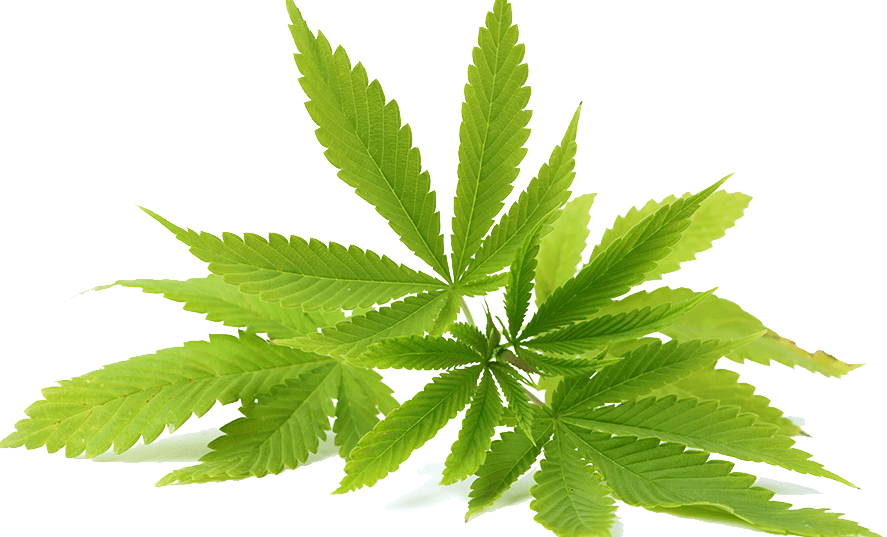
\includegraphics[width=200pt]{images/organik_bro} 
	
	\caption{Sayuran Organik}                         % Label gambar
\end{figure}
	\end{minted}

	\begin{figure}[!ht]                                  % [!ht] sebagai floatifier really here-top
		\centering                                       % Menengahkan gambar
		
		% Tampilkan dalam ukuran lebar 200pt gambar image/organik_bro
		% Pastikan berkas gambar atau foldernya di folder yang sama dengan berkas tex nya.
		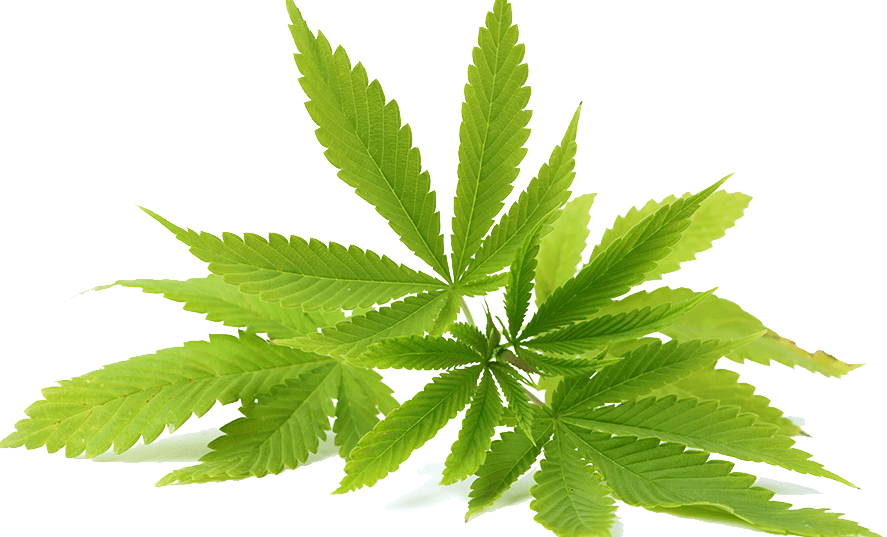
\includegraphics[width=200pt]{images/organik_bro} 
		
		\caption{Sayuran Organik}                         % Label gambar
	\end{figure}
	
	\newpage
	
	Dapat pula menggunakan beberapa gambar menjadi dalam satu lingkungan
	menggunakan lingkungan \textbf{subfigure}.
	
	Tambahkan paket \textbf{subcaption} untuk dapat menggunakan \textbf{subfigure}
	
	\begin{minted}[frame=lines,framesep=2mm,fontsize=\normalsize,bgcolor=LightGray]{tex}
\usepackage{subcaption}
	\end{minted}
	
	Sebagai contoh:
	\begin{minted}[frame=lines,framesep=2mm,fontsize=\normalsize,bgcolor=LightGray]{tex}
\begin{figure}[!ht]
	\centering
	\begin{subfigure}[t]{0.25\textwidth}
		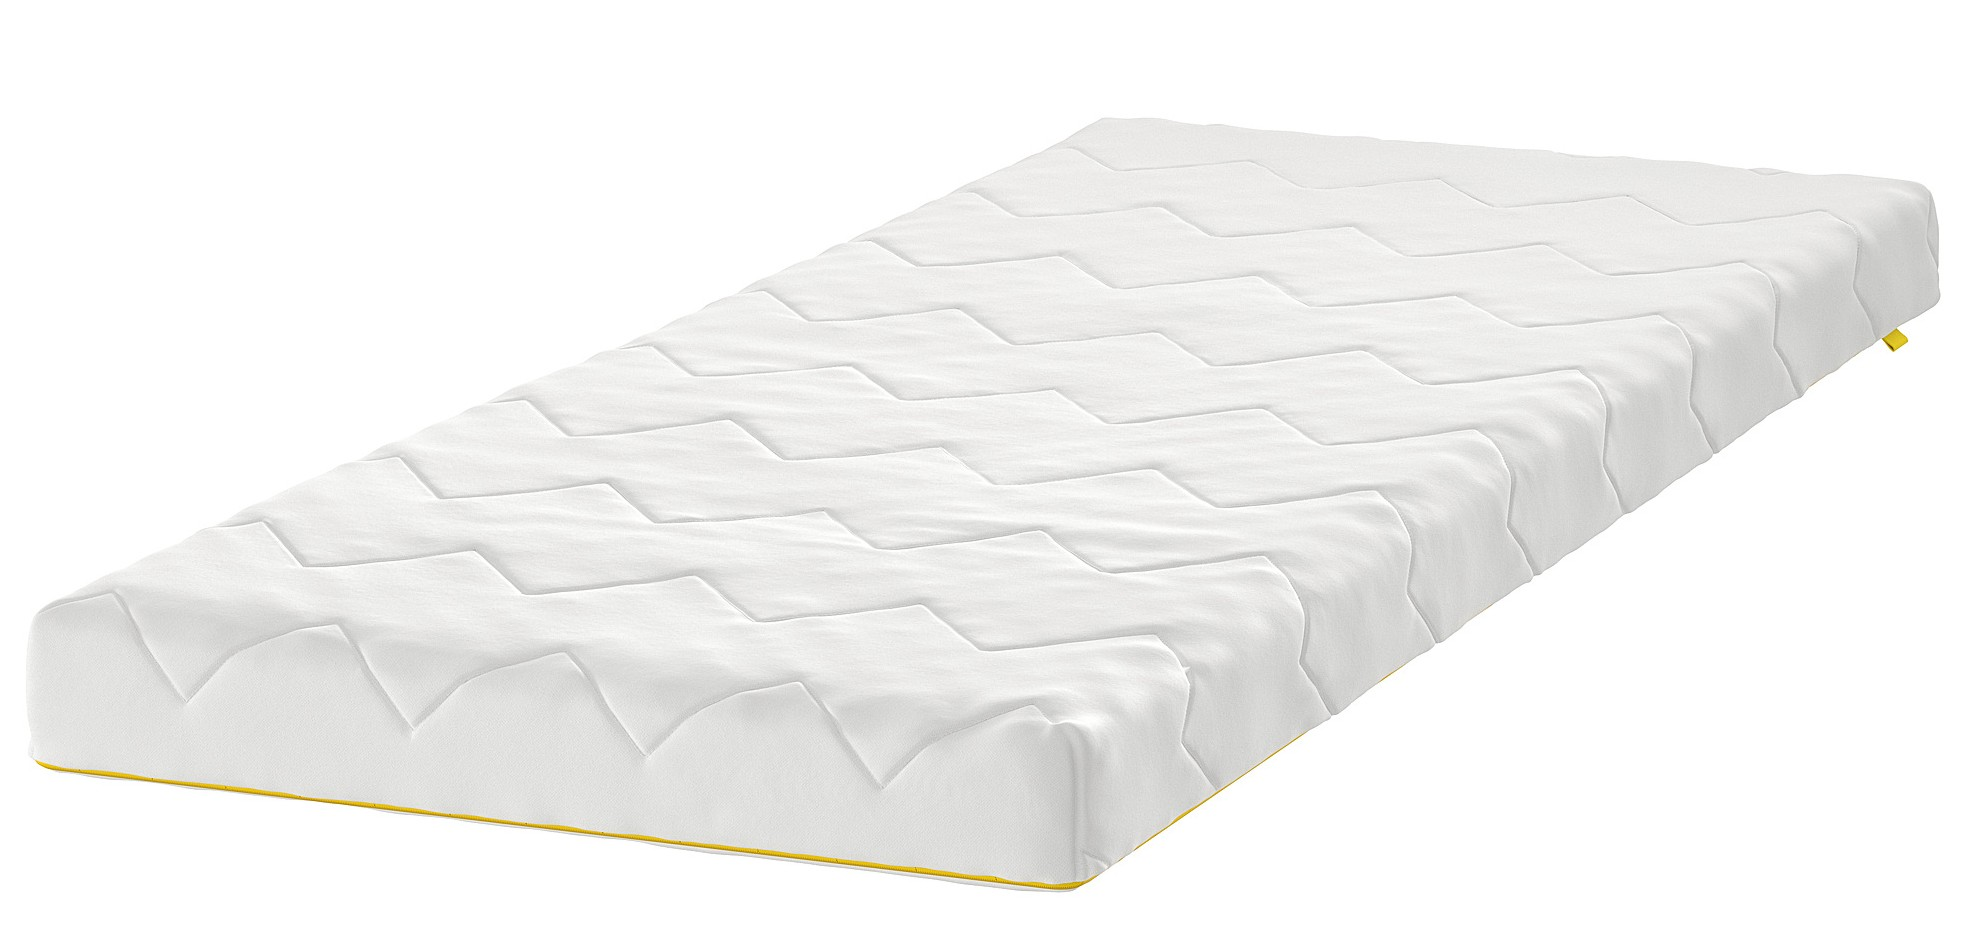
\includegraphics[width=\textwidth]{images/apo1}
		\caption{Kasur}
	\end{subfigure}

	\begin{subfigure}[t]{0.25\textwidth}
		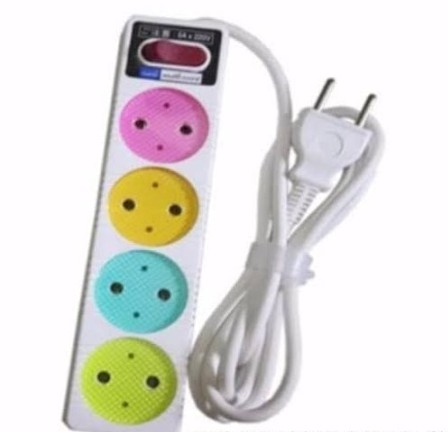
\includegraphics[width=\textwidth]{images/apo2}
		\caption{Listrik}
	\end{subfigure}
	\\ % garis baru agar terbagi dalam 2 baris
	\begin{subfigure}[t]{0.25\textwidth}
		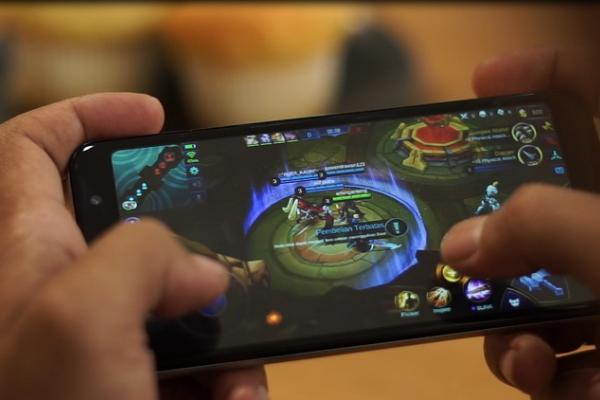
\includegraphics[width=\textwidth]{images/apo3}
		\caption{Game Bocah}
	\end{subfigure}

	\begin{subfigure}[t]{0.25\textwidth}
		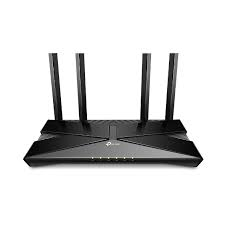
\includegraphics[width=\textwidth]{images/apo4}
		\caption{WiFi Indi-Home}
	\end{subfigure}

	\caption{Four Horseman of Apocalypse}
\end{figure}
	\end{minted}

	Hasilnya:
	
	\begin{figure}[!ht]
		\centering
		\begin{subfigure}[t]{0.25\textwidth}
			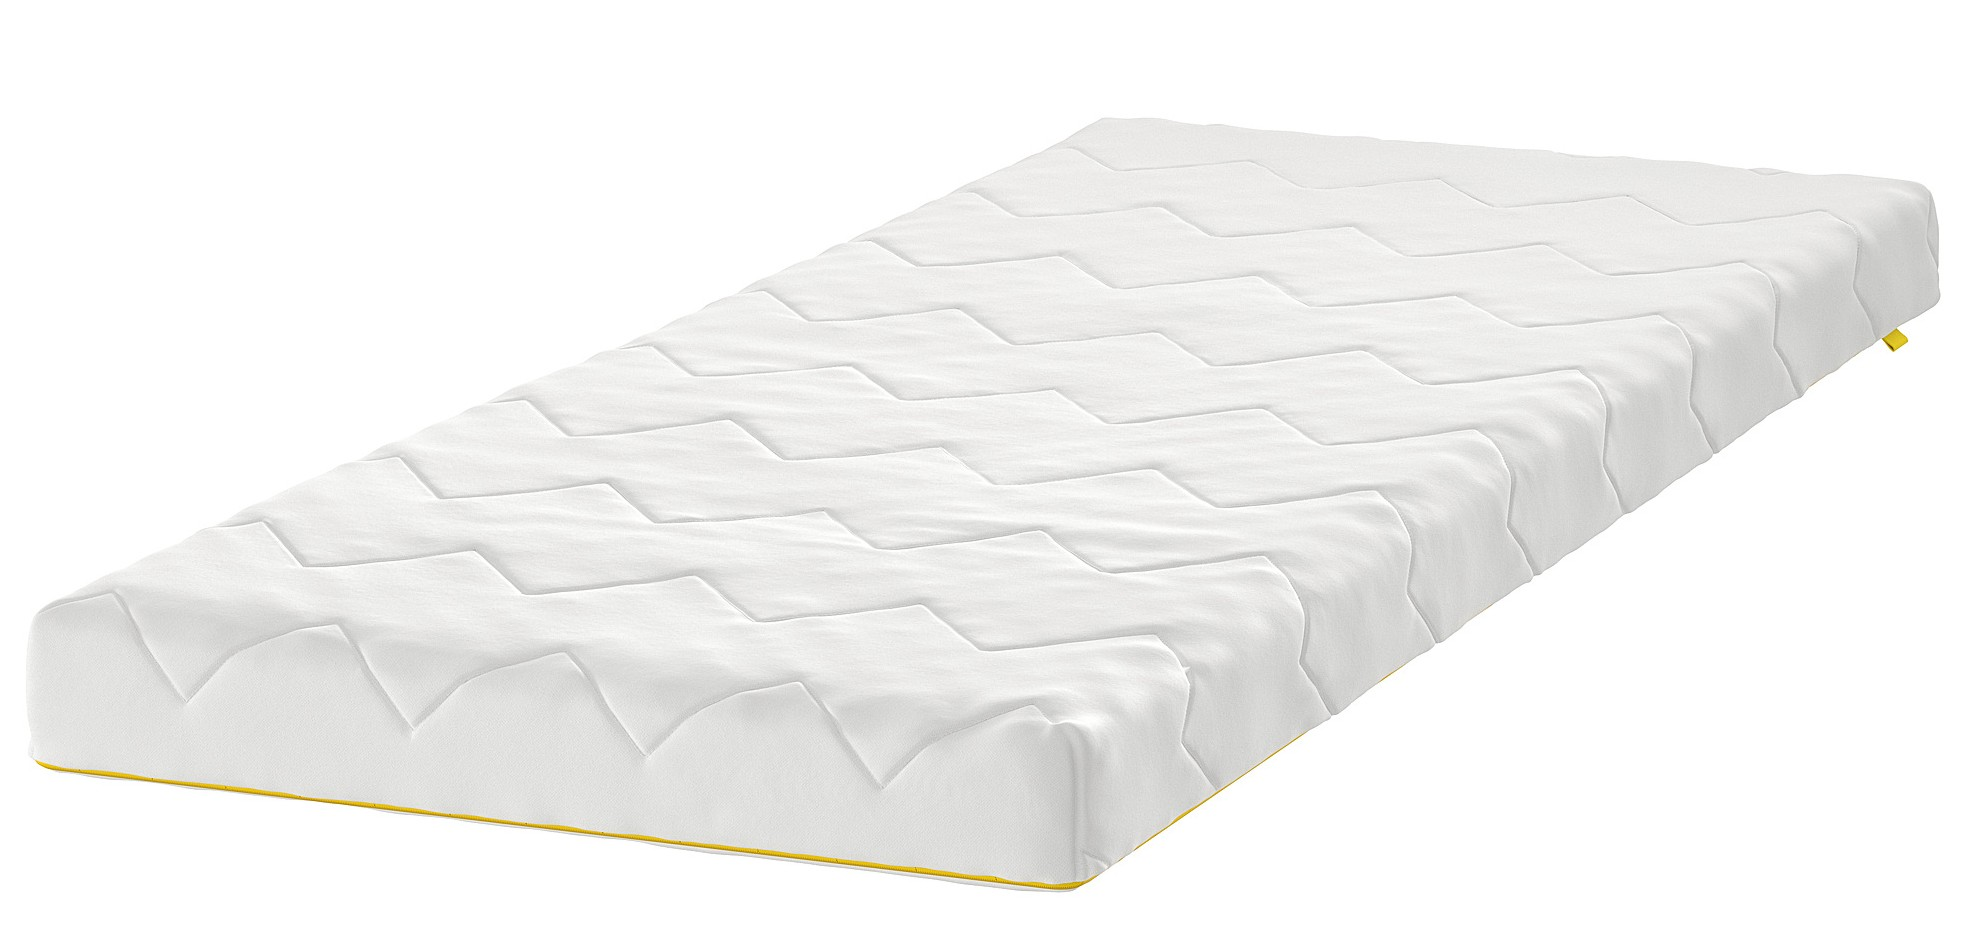
\includegraphics[width=\textwidth]{images/apo1}
			\caption{Kasur}
		\end{subfigure}
		\begin{subfigure}[t]{0.25\textwidth}
			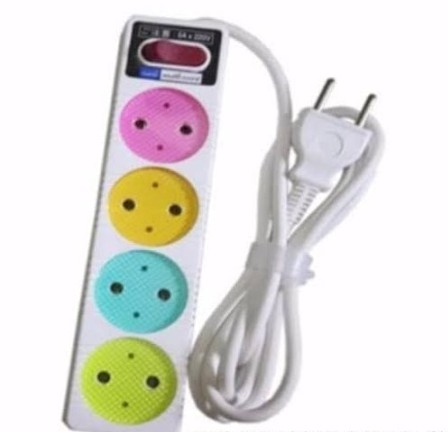
\includegraphics[width=\textwidth]{images/apo2}
			\caption{Listrik}
		\end{subfigure}
		\\
		\begin{subfigure}[t]{0.25\textwidth}
			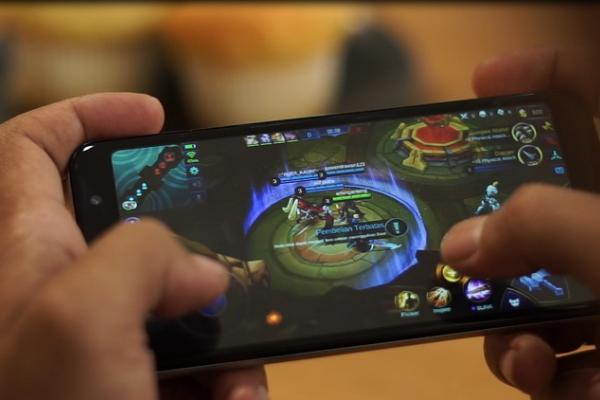
\includegraphics[width=\textwidth]{images/apo3}
			\caption{Game Bocah}
		\end{subfigure}
		\begin{subfigure}[t]{0.25\textwidth}
			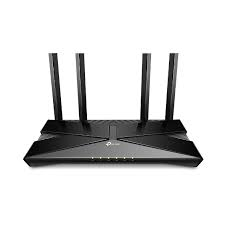
\includegraphics[width=\textwidth]{images/apo4}
			\caption{WiFi Indi-Home}
		\end{subfigure}
	
		\caption{Four Horseman of Apocalypse}
	\end{figure}
	
	\newpage
	\section{Table}
	
	\subsection{Manual}
	
	Untuk menulis tabel secara manual, bentuknya mirip dengan membuat matrix,
	dengan lingkungan \textbf{table} dan \textbf{tabular} (bukan matematis) yang ditambahkan header dan garis.
	Tabel dapat ditulis di dalam lingkungan \textbf{center} agar dapat mentengahkan tabel.
	
	Untuk mempermudah membuat garis tabel dan mengganti label menjadi "Tabel", tambahkan pengaturan berikut sebelum lingkungan \textbf{document}.
	\begin{minted}[frame=lines,framesep=2mm,fontsize=\normalsize,bgcolor=LightGray]{tex}
\usepackage{booktabs}
\addto\captionsenglish{\renewcommand{\tablename}{Tabel}}
	\end{minted}

	Berikut contoh membuat tabel.
	\begin{minted}[frame=lines,framesep=2mm,fontsize=\normalsize,bgcolor=LightGray]{tex}
\begin{table}[h!]
	\begin{center}
		\begin{tabular}{ |c|c|c| } 
			\toprule
			Person & Strength & Weakness \\ 
			\midrule
			Spongebob & Optimistic & Unrealistic \\ 
			Patrick & Dumb & Troublemaker \\
			Squidward & Realistic & Narcistic \\
			\bottomrule
		\end{tabular}
		\caption{Favorite Anime Characters}	
	\end{center}
\end{table}
	\end{minted}

	Akan menghasilkan:
	
	\begin{table}[h!]
		\begin{center}
			\begin{tabular}{ |c|c|c| } 
				\toprule
				Person & Strength & Weakness \\ 
				\midrule
				Spongebob & Optimistic & Unrealistic \\ 
				Patrick & Dumb & Troublemaker \\
				Squidward & Realistic & Narcistic \\
				\bottomrule
			\end{tabular}
			\caption{Favorite Anime Characters}	
		\end{center}
	\end{table}

	Jika membutuhkan multi kolom, tambahkan paket \textbf{multirow}
	\begin{minted}[frame=lines,framesep=2mm,fontsize=\normalsize,bgcolor=LightGray]{tex}
\usepackage{multirow}
	\end{minted}

	Berikut contohnya:	
	\begin{minted}[frame=lines,framesep=2mm,fontsize=\normalsize,bgcolor=LightGray]{tex}
\begin{table}[h!]
	\begin{center}
		\begin{tabular}{ |c|c|c| } 
			\toprule
			Person & Strength & Weakness \\ 
			\midrule
			Spongebob & Optimistic & Unrealistic \\ 
			Patrick & Dumb & Troublemaker \\
			Squidward & Realistic & Narcistic \\
			Mr.Krabs & \multicolumn{2}{c|}{Money Oriented} \\ 
			\bottomrule
		\end{tabular}
		\caption{Favorite Anime Characters}	
	\end{center}
\end{table}
	\end{minted}

	\newpage
	Akan menghasilkan:
	
	\begin{table}[h!]
		\begin{center}
			\begin{tabular}{ |c|c|c| } 
				\toprule
				Person & Strength & Weakness \\ 
				\midrule
				Spongebob & Optimistic & Unrealistic \\ 
				Patrick & Dumb & Troublemaker \\
				Squidward & Realistic & Narcistic \\
				Mr.Krabs & \multicolumn{2}{c|}{Money Oriented} \\ 
				\bottomrule
			\end{tabular}
			\caption{Favorite Anime Characters}	
		\end{center}
	\end{table}
	
	\subsection{Impor CSV}
	
	Jika tabel digunakan untuk menampilkan banyak baris data, maka menulis tabel secara manual akan sangat memakan waktu.
	Untuk itu, dapat digunakan paket \textbf{pgfplotstable} untuk melakukan impor data dari suatu berkas CSV (Comma Separated Value).
	Paket \textbf{booktabs} dapat dipakai untuk mempermudah membuat garis pemisah (seperti sebelumnya).

	\begin{minted}[frame=lines,framesep=2mm,fontsize=\normalsize,bgcolor=LightGray]{tex}
\usepackage{pgfplotstable, booktabs}
	\end{minted}

	Contoh suatu berkas CSV pendek (harus tanpa header) berisi daftar komponen digital, disimpan sebagai \textbf{bom.csv}:
	\begin{minted}[frame=lines,framesep=2mm,fontsize=\normalsize,bgcolor=LightGray]{text}
1;"U1,U4";"QFN-16-1EP_3x3mm_P0.5mm_EP1.7x1.7mm";2;"MAX98357";;;
2;"U2";"LQFP-64_10x10mm_P0.5mm";1;"STM32F401RETx";;;
3;"U3";"SOT-223-3_TabPin2";1;"AMS1117-3.3";;;
4;"U5";"ESP-12E";1;"ESP-12E";;;
5;"U6";"sph0645";1;"SPH0645";;;
	\end{minted}

	Berikut contoh impor CSV tersebut menjadi tabel (lingkungan \textbf{tabular} diganti menjadi tag \textbf{pgfplotstable}):
	
	\begin{minted}[frame=lines,framesep=2mm,fontsize=\normalsize,bgcolor=LightGray]{tex}
\begin{table}[h!]
	\begin{center}
		\pgfplotstabletypeset[
		col sep = semicolon,             % tanda titik-koma sebagai pemisah nilai
		string replace*={_}{\_},         % agar '_' tetap dianggap '_' (bukan subscript)
		string replace*={"}{},           % agar tanda dobel petik dianggap tidak ada
		header=false,                    % agar baris pertama file CSV tidak dianggap header
		display columns/0/.style={string type,column name={Id}},          % kolom 0
		display columns/1/.style={string type,column name={Designator}},  % kolom 1
		display columns/2/.style={string type,column name={Package}},     % kolom 2
		display columns/3/.style={string type,column name={Quantity}},    % kolom 3
		display columns/4/.style={string type,column name={Designation}}, % kolom 4
		every head row/.style={before row=\toprule,after row=\midrule},   % garis header
		every last row/.style={after row=\bottomrule},                    % garis bawah
		]{files/bom.csv}                                                  % nama file CSV
		\caption{Bill of Material (Digital parts)}	
	\end{center}
\end{table}
	\end{minted}

	akan menghasilkan:
	
	\begin{table}[h!]
		\begin{center}
			\pgfplotstabletypeset[
			col sep = semicolon,             % tanda titik-koma sebagai pemisah nilai
			string replace*={_}{\_},         % agar '_' tetap dianggap '_' (bukan subscript)
			string replace*={"}{},           % agar tanda dobel petik dianggap tidak ada
			header=false,                    % agar baris pertama file CSV tidak dianggap header
			display columns/0/.style={string type,column name={Id}},          % kolom 0
			display columns/1/.style={string type,column name={Designator}},  % kolom 1
			display columns/2/.style={string type,column name={Package}},     % kolom 2
			display columns/3/.style={string type,column name={Quantity}},    % kolom 3
			display columns/4/.style={string type,column name={Designation}}, % kolom 4
			every head row/.style={before row=\toprule,after row=\midrule},   % garis header
			every last row/.style={after row=\bottomrule},                    % garis bawah
			]{files/bom.csv}                                                  % nama file CSV
			\caption{Bill of Material (Digital parts)}	
		\end{center}
	\end{table}

	\newpage
	\section{Diagram/Plot}
	
	\LaTeX{} menyediakan paket untuk membuat gambar tipe vektor baik untuk diagram maupun plot.
	Salah satu paket yang umum digunakan adalah \textbf{tikz}.
	
	\begin{minted}[frame=lines,framesep=2mm,fontsize=\normalsize,bgcolor=LightGray]{tex}
\usepackage{tikz}
	\end{minted}
	
	\subsection{Diagram}
	
	Berikut contoh menggambar diagram dengan paket \textbf{tikz}.
	Lingkungan yang digunakan sama dengan gambar (\textbf{figure}), namun ditambahkan lingkungan \textbf{tikzpicture}.
	
	\begin{minted}[frame=lines,framesep=2mm,fontsize=\normalsize,bgcolor=LightGray]{tex}
\begin{figure}[!ht]
	\begin{center}
		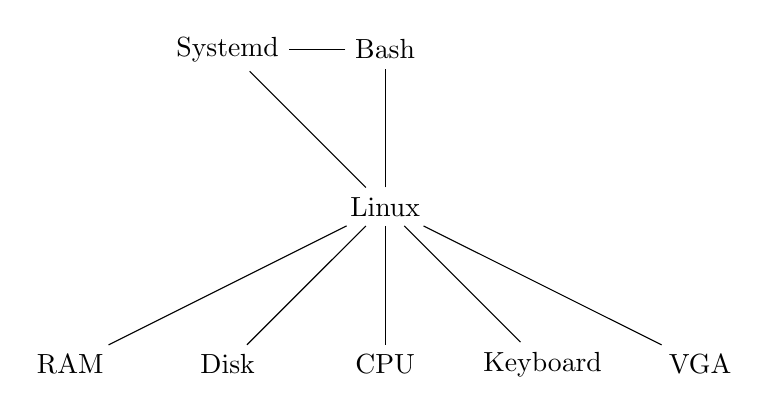
\begin{tikzpicture}[node distance=2cm]
			% definisi untuk node
			% \node nama [posisi] {text};             % jangan lupa titik-koma !
			\node (linux) [] {Linux};                 % posisi acuan
			\node (bash) [above of=linux] {Bash};     % di atas acuan
			\node (systemd) [left of=bash] {Systemd}; % di kiri sebelumnya
			\node (cpu) [below of=linux] {CPU};       % di bawah acuan
			\node (ram) [left of=cpu] {Disk};         % di kiri sebelumnya
			\node (disk) [left of=ram] {RAM};         % di kiri sebelumnya
			\node (key) [right of=cpu] {Keyboard};
			\node (vga) [right of=key] {VGA};

			
			% menggambar untuk garis koneksi
			% \draw [opsi] (nama) -- (nama);
			\draw [] (linux) -- (bash);
			\draw [] (linux) -- (systemd);
			\draw [] (bash) -- (systemd);
			\draw [] (linux) -- (cpu);
			\draw [] (linux) -- (ram);
			\draw [] (linux) -- (disk);
			\draw [] (linux) -- (key);
			\draw [] (linux) -- (vga);
		\end{tikzpicture}
		\caption{Diagram Struktur Minimum Sistem Operasi Linux}
	\end{center}
\end{figure}
	\end{minted}
	
	menghasilkan:
	
	\begin{figure}[!ht]
		\begin{center}
			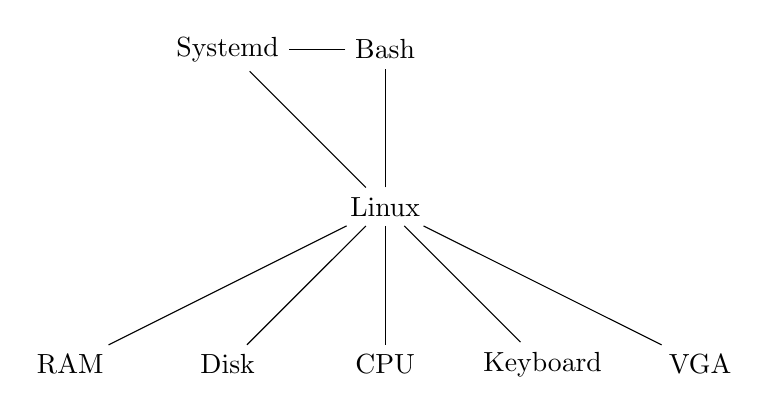
\begin{tikzpicture}[node distance=2cm]
				% definisi untuk node
				% \node nama [posisi] {text};             % jangan lupa titik-koma !
				\node (linux) [] {Linux};                 % posisi acuan
				\node (bash) [above of=linux] {Bash};     % di atas acuan
				\node (systemd) [left of=bash] {Systemd}; % di kiri sebelumnya
				\node (cpu) [below of=linux] {CPU};       % di bawah acuan
				\node (ram) [left of=cpu] {Disk};         % di kiri sebelumnya
				\node (disk) [left of=ram] {RAM};         % di kiri sebelumnya
				\node (key) [right of=cpu] {Keyboard};
				\node (vga) [right of=key] {VGA};

				
				% menggambar untuk garis koneksi
				% \draw [opsi] (nama) -- (nama);
				\draw [] (linux) -- (bash);
				\draw [] (linux) -- (systemd);
				\draw [] (bash) -- (systemd);
				\draw [] (linux) -- (cpu);
				\draw [] (linux) -- (ram);
				\draw [] (linux) -- (disk);
				\draw [] (linux) -- (key);
				\draw [] (linux) -- (vga);
			\end{tikzpicture}
			\caption{Diagram Struktur Minimum Sistem Operasi Linux}
		\end{center}
	\end{figure}
	
	Kemudian dapat pula ditambahkan pengaturan lebih lanjut (sebelum lingkungan \textbf{document}) untuk memodifikasi objek diagram.
	Berikut contoh memodifikasi kotak, dan garis diagram:
	
	\begin{minted}[frame=lines,framesep=2mm,fontsize=\normalsize,bgcolor=LightGray]{tex}
\tikzstyle{squared} = [rectangle, rounded corners, minimum width=1cm, minimum height=0.5cm,text centered, draw=black]
\tikzstyle{connect1} = [ultra thick,->]
\tikzstyle{connect2} = [ultra thick,<->]
	\end{minted}

	dan contoh implementasi:
	
	\begin{minted}[frame=lines,framesep=2mm,fontsize=\normalsize,bgcolor=LightGray]{tex}
\begin{figure}[!ht]
	\begin{center}
		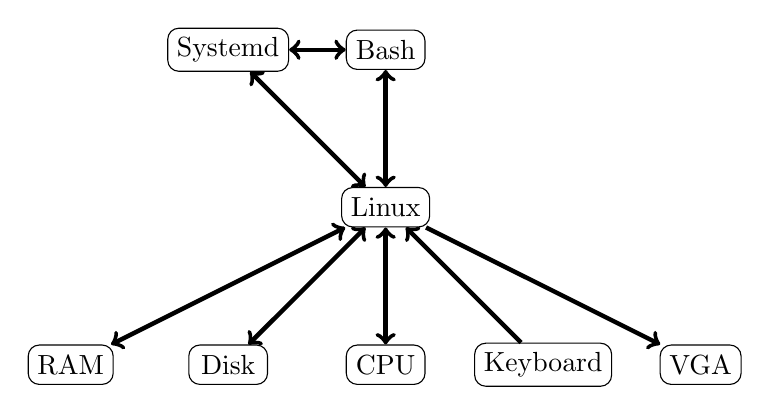
\begin{tikzpicture}[node distance=2cm]
			% definisi untuk node
			% \node nama [squared, posisi] {text};             % jangan lupa titik-koma !
			\node (linux) [squared] {Linux};                   % posisi acuan
			\node (bash) [squared, above of=linux] {Bash};     % di atas acuan
			\node (systemd) [squared, left of=bash] {Systemd}; % di kiri sebelumnya
			\node (cpu) [squared, below of=linux] {CPU};       % di bawah acuan
			\node (ram) [squared, left of=cpu] {Disk};         % di kiri sebelumnya
			\node (disk) [squared, left of=ram] {RAM};         % di kiri sebelumnya
			\node (key) [squared, right of=cpu] {Keyboard};
			\node (vga) [squared, right of=key] {VGA};

			
			% menggambar untuk garis koneksi
			% \draw [connectX] (nama) -- (nama);
			\draw [connect2] (linux) -- (bash);
			\draw [connect2] (linux) -- (systemd);
			\draw [connect2] (bash) -- (systemd);
			\draw [connect2] (linux) -- (cpu);
			\draw [connect2] (linux) -- (ram);
			\draw [connect2] (linux) -- (disk);
			\draw [connect1] (key) -- (linux);
			\draw [connect1] (linux) -- (vga);
		\end{tikzpicture}
		\caption{Diagram Struktur Minimum Sistem Operasi Linux}
	\end{center}
\end{figure}
	\end{minted}
	
	menghasilkan:
	
	\begin{figure}[!ht]
		\begin{center}
			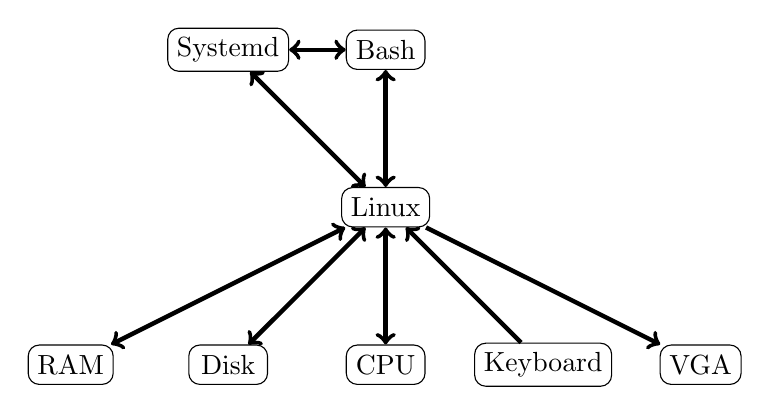
\begin{tikzpicture}[node distance=2cm]
				% definisi untuk node
				% \node nama [squared, posisi] {text};             % jangan lupa titik-koma !
				\node (linux) [squared] {Linux};                   % posisi acuan
				\node (bash) [squared, above of=linux] {Bash};     % di atas acuan
				\node (systemd) [squared, left of=bash] {Systemd}; % di kiri sebelumnya
				\node (cpu) [squared, below of=linux] {CPU};       % di bawah acuan
				\node (ram) [squared, left of=cpu] {Disk};         % di kiri sebelumnya
				\node (disk) [squared, left of=ram] {RAM};         % di kiri sebelumnya
				\node (key) [squared, right of=cpu] {Keyboard};
				\node (vga) [squared, right of=key] {VGA};

				
				% menggambar untuk garis koneksi
				% \draw [connectX] (nama) -- (nama);
				\draw [connect2] (linux) -- (bash);
				\draw [connect2] (linux) -- (systemd);
				\draw [connect2] (bash) -- (systemd);
				\draw [connect2] (linux) -- (cpu);
				\draw [connect2] (linux) -- (ram);
				\draw [connect2] (linux) -- (disk);
				\draw [connect1] (key) -- (linux);
				\draw [connect1] (linux) -- (vga);
			\end{tikzpicture}
			\caption{Diagram Struktur Minimum Sistem Operasi Linux}
		\end{center}
	\end{figure}
	
	\subsection{Plot}
	
	Selain diagram, paket \textbf{tikz} juga dapat digunakan untuk menggambar plot atau grafik matematis.
	Dengan menambahkan paket \textbf{pgfplots}, kita dapat pula melakukan impor berkas CSV
	dan melakukan plot menggunakan \textbf{tikz} berdasarkan hasil impor sebelumnya.
	Tambahkan dulu kedua paket tersebut:
	
	\begin{minted}[frame=lines,framesep=2mm,fontsize=\normalsize,bgcolor=LightGray]{tex}
\usepackage{tikz, pgfplots}
	\end{minted}
	
	Untuk kebutuhan contoh, berikut program pendek Python/NumPy yang dapat digunakan untuk membuat CSV sederhana:
	\begin{minted}[frame=lines,framesep=2mm,fontsize=\normalsize,bgcolor=LightGray]{python}
#/usr/bin/python
import numpy as np
import matplotlib.pyplot as plt
x = np.around(np.linspace(0,1,20), decimals=2)
y = np.around(np.sin(x), decimals=2)
z = np.transpose((x,y))
np.savetxt('coba.csv', z, delimiter=';',fmt='%5.2f')
plt.plot(x,y)
plt.show()
	\end{minted}

	Jalankan skrip python di atas, maka akan didapat berkas \textbf{coba.csv}.
	Selain akan didapat pula grafik matplotlib seperti ini:
	
	\begin{figure}[!ht]                                  
		\centering
		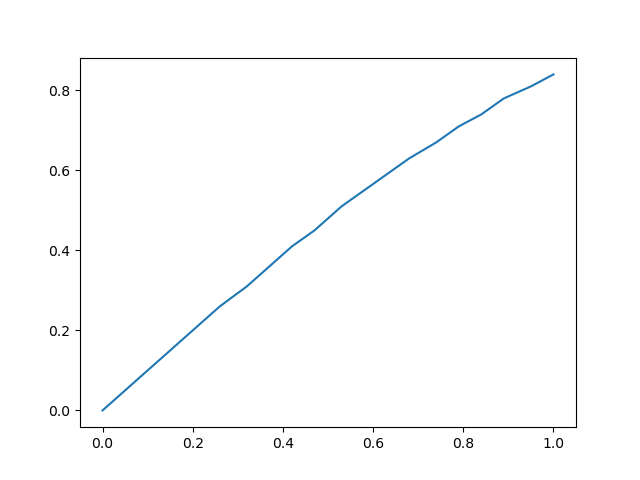
\includegraphics[width=150pt]{images/cobacsv}
		\caption{Contoh Plot dengan Matplotlib}     
	\end{figure}

	sedangkan menggunakan \textbf{tikz} dan \textbf{pgfplots} dengan lingkungan \textbf{axis}, berikut contohnya:

	\begin{minted}[frame=lines,framesep=2mm,fontsize=\normalsize,bgcolor=LightGray]{tex}
\begin{figure}[!ht]
	\centering
	\begin{tikzpicture}
		\begin{axis}[
			grid=major,                   % tampilkan grid
			%grid style={dashed,gray!30}, % pengaturan grid
			table/col sep=semicolon,      % tanda titik-koma sebagai pemisah nilai
			width=0.3\textwidth,         % lebar gambar 30% halaman
			]\addplot table[              % plot dari tabel
			x index = {0},                % x dari kolom ke 0
			y index = {1}                 % y dari kolom ke 1
			] {files/coba.csv};           % file sumber. Jangan lupa titik-koma !
		\end{axis}
	\end{tikzpicture}
	\caption{Plot langsung dari CSV}
\end{figure}
	\end{minted}
	
	akan menghasilkan

	\begin{figure}[!ht]
		\centering
		\begin{tikzpicture}
			\begin{axis}[
					grid=major,                   % tampilkan grid
					%grid style={dashed,gray!30}, % pengaturan grid
					table/col sep=semicolon,      % tanda titik-koma sebagai pemisah nilai
					width=0.3\textwidth,          % lebar gambar 30% halaman
				]\addplot table[                  % plot dari tabel
					x index = {0},                % x dari kolom ke 0
					y index = {1}                 % y dari kolom ke 1
				] {files/coba.csv};               % file sumber. Jangan lupa titik-koma !
			\end{axis}
		\end{tikzpicture}
		\caption{Plot langsung dari CSV}
	\end{figure}
	
	\newpage
	\section{Daftar Isi/Gambar/Tabel}
	
	Sebelum menggunakan fitur daftar isi/gambar tabel,
	pastikan menambahkan paket \textbf{tocbibind} agar semua daftar dapat terdaftar di ToC itu sendiri.
	
	\begin{minted}[frame=lines,framesep=2mm,fontsize=\normalsize,bgcolor=LightGray]{tex}
\usepackage{tocbibind}
	\end{minted}
	
	\subsection{Halaman Daftar}
	
	Untuk menyisipkan halaman-halaman daftar, berikut contoh:
	
	\begin{minted}[frame=lines,framesep=2mm,fontsize=\normalsize,bgcolor=LightGray]{tex}
\newpage % halaman baru
\tableofcontents % daftar isi
\listoffigures % daftar gambar
\listoftables % daftar table
	\end{minted}

	\textbf{TIPS:} Walaupun tidak ada tag \textbf{newpage} di antara halaman-halaman daftar,
	\LaTeX{} sudah otomatis memisahkan setiap halaman daftar di halaman baru.

	\subsection{Mengganti Label}
	
	Untuk menyesuaikan label halaman daftar, dapat digunakan pengaturan-pengaturan berikut (sebelum lingkungan \textbf{document}):
	
	\begin{minted}[frame=lines,framesep=2mm,fontsize=\normalsize,bgcolor=LightGray]{tex}
% Mengganti label "Contents" ke "Daftar Isi"
\addto\captionsenglish{\renewcommand{\contentsname}{Daftar Isi}}

% Mengganti label "List of Figures" ke "Daftar Gambar"
\addto\captionsenglish{\renewcommand{\listfigurename}{Daftar Gambar}}

% Mengganti label "List of Tables" ke "Daftar Table"
\addto\captionsenglish{\renewcommand{\listtablename}{Daftar Tabel}}
	\end{minted}
	
	\section{Catatan Kaki}
	
	Untuk menambah catatan kaki, digunakan tag \textbf{footnote} dan \textbf{label}.
	Kemudian dapat pula menggunakan tag \textbf{ref} untuk menyebutkan catatan kaki.
	Penomoran catatan kaki otomatis diatur oleh kompiler \LaTeX.
	
	Contoh:
	
	\begin{minted}[frame=lines,framesep=2mm,fontsize=\normalsize,bgcolor=LightGray]{tex}
Lorem ipsum dolor sit amet, consectetur adipiscing elit.
Maecenas fringilla ut nunc sed cursus.
\footnote{\label{firstnote}Teks ini tidak memiliki arti yang koheren}.

Menurut suatu grimoire\footnote{\label{secondnote}buku kumpulan mantra latin},
teks latin ini adalah \textit{sigil words}\footnote{\label{thirdnote}pemanggil entitas metafisika}
walaupun tidak demikian sebagaimana catatan \ref{firstnote}.
	\end{minted}

	Hasilnya:
	
	\bigskip
	
	Lorem ipsum dolor sit amet, consectetur adipiscing elit.
	Maecenas fringilla ut nunc sed cursus.
	\footnote{\label{firstnote}Teks ini tidak memiliki arti yang koheren}.
	
	Menurut suatu grimoire\footnote{\label{secondnote}buku kumpulan mantra latin},
	teks latin ini adalah \textit{sigil words}\footnote{\label{thirdnote}pemanggil entitas metafisika}
	walaupun tidak demikian sebagaimana catatan \ref{firstnote}.
	
	\newpage
	\section{Bibliografi}
	
	\LaTeX{} mendukung penulisan daftar pustaka yang biasa disebut \textbf{BibTeX}.
	Suatu berkas BibTeX berisi metadata sebuah publikasi.
	Untuk membuat berkas BibTex, dapat dibuat dengan cara manual atau otomatis via Mendeley dan semacamnya.
	
	Untuk menambah fungsionalitas, dapat ditambahkan pake \textbf{babel} yang diatur ke bahasa \textbf{english}:
	
	\begin{minted}[frame=lines,framesep=2mm,fontsize=\normalsize,bgcolor=LightGray]{tex}
\usepackage[english]{babel}
	\end{minted}

	\subsection{Manual}
	
	Berikut contoh isi suatu berkas Bibtex sederhana, disimpan sebagai \textbf{contohbibtex.bib}:
	
	\begin{minted}[frame=lines,framesep=2mm,fontsize=\normalsize,bgcolor=LightGray]{tex}
@book{johndoe2100,
	AUTHOR="John Doe",
	TITLE="The Book without Title",
	PUBLISHER="Dummy Publisher",
	YEAR="2100",
}
@article{doejohn2500,
	AUTHOR="Doe John",
	TITLE="The Article without Title",
	PUBLISHER="Dummy Publisher",
	YEAR="2500",
}
	\end{minted}

	Kemudian berikut contoh dokumen dengan sitasi dan daftar pustaka (disimpan sebagai \textbf{cobabib.tex}):
	
	\begin{minted}[frame=lines,framesep=2mm,fontsize=\normalsize,bgcolor=LightGray]{tex}
\documentclass{article}

\usepackage[english]{babel}

\begin{document}
	Membaca buku kabarnya menyenangkan \cite{johndoe2100},  % sitasi dengan key metadata
	tapi nyatanya selalu berakhir pusing \cite{doejohn2500}.
	
	\newpage
	\bibliographystyle{IEEEtran}  % model penulisan daftar pustaka
	\bibliography{contohbibtext}  % berkas bibtex (ditulis tanpa ekstensi *.bib)
\end{document}
	\end{minted}

	Untuk kompilasi di command-line (di luar TexStudio), perlu dilakukan beberapa langkah.
	Berikut perintah secara berurutan:

	\begin{minted}[frame=lines,framesep=2mm,fontsize=\normalsize,bgcolor=LightGray]{tex}
pdflatex -shell-escape -synctex=1 -interaction=nonstopmode cobabib.tex
bibtex cobabib.aux
pdflatex -shell-escape -synctex=1 -interaction=nonstopmode cobabib.tex
pdflatex -shell-escape -synctex=1 -interaction=nonstopmode cobabib.tex
	\end{minted}

	Namun jika menggunakan editor seperti TexStudio, sudah akan terkompile dengan sendirinya.
	
	\bigskip
	
	\textbf{TIPS:} Untuk mengganti label "References" ke "Daftar Pustaka", tambahkan pengaturan berikut sebelum lingkungan \textbf{document}.
	
	\begin{minted}[frame=lines,framesep=2mm,fontsize=\normalsize,bgcolor=LightGray]{tex}
\addto\captionsenglish{\renewcommand{\bibname}{Daftar Pustaka}} % untuk book atau report
	\end{minted}

	sedangkan khusus untuk kelas dokumen \textbf{article}:
	
	\begin{minted}[frame=lines,framesep=2mm,fontsize=\normalsize,bgcolor=LightGray]{tex}
\addto\captionsenglish{\renewcommand{\refname}{Daftar Pustaka}} % untuk article
	\end{minted}
	
	\newpage
	\subsection{Mendeley}
	
	Software References Manager seperti Mendeley juga dapat digunakan untuk membuat berkas bibtex secara otomatis.
	Berikut langkah-langkahnya:
	\begin{enumerate}
		\item Klik menu \textit{Tools} -> \textit{Options}.
		\item Pilih tab \textbf{BibTex}.
		\item Centang beberapa opsi berikut:
		\begin{itemize}
			\item Excape LaTeX special characters
			\item Use Journal Abbreviatons
			\item Enable BibTeX syncing
		\end{itemize}
		\item Untuk pilihan scope, ambil \textit{for my whole library}.
		\item Untuk Path, pilih sesuka hati (disini contoh \textbf{'/home/achmaday/Documents'}).
	\end{enumerate}
	
	\begin{figure}[!ht]                                  
		\centering
		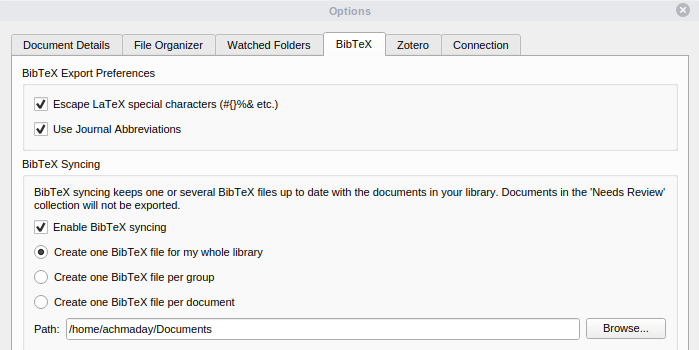
\includegraphics[width=400pt]{images/mendeley_bibtex}
		\caption{Opsi BibTeX di Mendeley}     
	\end{figure}

	Setelah diklik \textbf{Apply} dan \textbf{Ok}, maka di alamat Path akan tersedia berkas \textbf{library.bib}.
	
	\bigskip
	
	Berikut contoh dokumen
	
	\begin{minted}[frame=lines,framesep=2mm,fontsize=\normalsize,bgcolor=LightGray]{tex}
\documentclass{article}

\usepackage[english]{babel}

\begin{document}
	Membaca buku kabarnya menyenangkan \cite{Tian2017},  % sitasi dengan key metadata
	tapi nyatanya selalu berakhir pusing \cite{Electronics2005}.
	
	\newpage
	\bibliographystyle{IEEEtran}                     % model penulisan daftar pustaka
	\bibliography{/home/achmaday/Documents/library}  % alamat berkas bibtex menyesuaikan
\end{document}
	\end{minted}
	
	\newpage
	\section{Source Code}
	
	Untuk menuliskan kode sumber programming atau semacamnya, digunakan lingkungan \textbf{minted} dari paket \textbf{minted}.
	
	\begin{minted}[frame=lines,framesep=2mm,fontsize=\normalsize,bgcolor=LightGray]{tex}
\usepackage{minted}
	\end{minted}

	Berikut contoh penulisan potongan kode Python:	
	
	\begin{verbatim}
\begin{minted}[fontsize=\normalsize]{python}
#!/usr/bin/python

import numpy as np
r = np.random.rand(3,2)
print(r)
\end{minted}
	\end{verbatim}

	\textbf{Perhatian:} Disini penulisan kode menggunakan \textbf{verbatim} agar dikompile sebagai teks apa adanya
	untuk menghindari kerancuan akibat minted bersarang.

	\bigskip
	
	Kode diatas akan menghasilkan:
	
	\begin{minted}[fontsize=\normalsize]{python}
#!/usr/bin/python

import numpy as np
r = np.random.rand(3,2)
print(r)
	\end{minted}

	Untuk menambahkan kotak latar, dapat menambahkan opsi \textbf{frame} (kotak):
	
	\begin{verbatim}
\begin{minted}[frame=lines,framesep=2mm,fontsize=\normalsize]{python}
#!/usr/bin/python

import numpy as np
r = np.random.rand(3,2)
print(r)
\end{minted}
	\end{verbatim}

	hasilnya:
	
	\begin{minted}[frame=lines,framesep=2mm,fontsize=\normalsize]{python}
#!/usr/bin/python

import numpy as np
r = np.random.rand(3,2)
print(r)
	\end{minted}
	
	%%%%%%%%%%%%%%%%%%%%%%%%%%%%%%%%%%%%%%%%%%%%%%%%%%%%%%%%%%%%%%%%%
	
	\newpage
	\chapter{Practical Templates}
	
	Coming Soon
	
	
	%%%%%%%%%%%%%%%%%%%%%%%%%%%%%%%%%%%%%%%%%%%%%%%%%%%%%%%%%%%%%%%%%
	
	\newpage
	\chapter{Presentasi Beamer}
	
	Coming Soon
	
	%%%%%%%%%%%%%%%%%%%%%%%%%%%%%%%%%%%%%%%%%%%%%%%%%%%%%%%%%%%%%%%%%
	
	\newpage
	\chapter{Git-SCM}
	
	\textbf{PERHATIAN:} Pembahasan bagian ini belum selesai !!!!
	
	Git SCM (Source Code Manager) adalah program untuk merekam dan tracking isi file (terutama file teks).
	Selain itu Git digunakan untuk mengolah modifikasi kode (patch) sehingga bisa diterapkan
	model pengembangan program yang bersifat kolaboratif.
	Mengingat kode sumber dokumen \LaTeX{} ditulis dalam format berkas teks,
	maka sangat cocok diterapkan Git SCM atau SCM lain untuk menulis \LaTeX{}.
	
	\textbf{PERHATIAN:} Bagian ini bukan merupakan pembahasan spesifik \LaTeX{}.
	Namun tool tambahan untuk mempermudah proses penulisan dokumen yang ditulis dengan instalasi \LaTeX{} offline.
	
	\section{Git-CLI}
	
	Berikut akan dibahas program Git CLI.
	Program ini adalah program utama Git yang berjalan di CLI (Command-Line Interface).
	
	\subsection{Instalasi}
	
	Berikut instalasi paket program Git:
	\begin{itemize}
		\item \textbf{Windows}. Download installer Windows Setup (jangan yang portable) disini:\\
		\url{https://git-scm.com/download/win}
		
		\item \textbf{ArchLinux/Manjaro}. Berikut perintah instalasi untuk distro ArchLinux/Manjaro dan turunannya:
		\begin{minted}[frame=lines,framesep=2mm,fontsize=\small,bgcolor=LightGray]{sh}
$> sudo pacman -S git tig
		\end{minted}
	\end{itemize}

	Disini versi yang digunakan sebagai acuan adalah Git-SCM untuk Windows.
	Untuk ArchLinux/Manjaro tinggal membuka terminal pada alamat folder yang akan digunakan untuk Git,
	dan tutorial selanjutnya akan sama baik perintah dan alur kerja untuk Windows maupun ArchLinux/Manjaro.

	\bigskip

	Selanjutnya buat folder baru kosong (contoh disini dinamai \textbf{git-coba}).
	Masuk ke folder tersebut, kemudian klik-kanan ruang kosong dalam folder tersebut.
	Kemudian pilih \textit{Git Bash Here}.
	
	\begin{figure}[!ht]
		\centering
		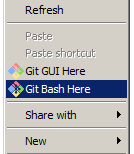
\includegraphics[width=100pt]{images/git/githere0}
		\caption{Konteks Menu Git Bash}
	\end{figure}

	\newpage
	Kemudian akan muncul jendela Git-CLI.
	Coba masukkan perintah berikut (tanda \textbf{\$} sebagai Prompt):
	\begin{minted}[frame=lines,framesep=2mm,fontsize=\small,bgcolor=LightGray]{sh}
$ git --version
	\end{minted}
	
	\begin{figure}[!ht]
		\centering
		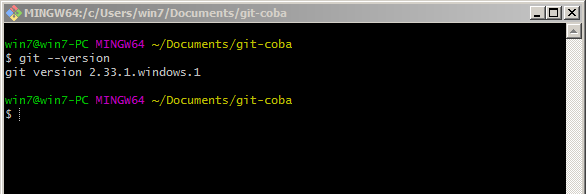
\includegraphics[width=400pt]{images/git/git0}
		\caption{Versi Git Terinstall}
	\end{figure}

	\subsection{Mendaftarkan ID}
	
	Sebelum melanjutkan, masukkan nama dan email agar Git bisa mencantumkan ID saat modifikasi kode.
	Contoh ID nama dan email penulis.
	\begin{minted}[frame=lines,framesep=2mm,fontsize=\small,bgcolor=LightGray]{sh}
$ git config --global user.name "Achmadi"
$ git config --global user.email "mekatronik.achmadi@gmail.com"
	\end{minted}

	\subsection{Git Repository}
	
	Selanjutnya untuk membuat repository Git baru, masukkan perintah CLI berikut di alamat folder \textbf{git-coba} tadi.
	\begin{minted}[frame=lines,framesep=2mm,fontsize=\small,bgcolor=LightGray]{sh}
$ git init
	\end{minted}
	
	\begin{figure}[!ht]
		\centering
		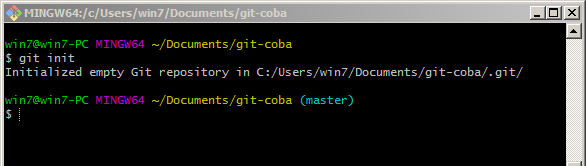
\includegraphics[width=400pt]{images/git/git1}
		\caption{Inisiasi Repo Git}
	\end{figure}
	
	Terlihat pada prompt CLI sekarang ditambahkan nama branch (master).
	Penjelasan term Branch dan cara Branching akan dibahas di bagian selanjutnya.
	
	\newpage
	Selain prompt yang berubah, juga akan muncul folder hidden \textbf{.git}.
	Jangan modifikasi isi folder ini kecuali melalui program Git.
	
	\begin{figure}[!ht]
		\centering
		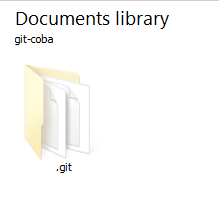
\includegraphics[width=150pt]{images/git/git2}
		\caption{Folder-Sistem Git}
	\end{figure}
	
\end{document}
